%% =====================================================================
%% Final Phase 2 ESA Report (covers Phase 1, Phase 2 and Phase 3)
%% AI-Assisted 3D Assembly Design
%% Parthasarathy Perumal -- M.Tech Data Science and AI, PES University
%% Built on the PES M.Tech project-report LaTeX template.
%% =====================================================================

%% oneside: one-sided printing (mandated by the submission checklist).
%% report defaults to oneside, but state it so a later class change can't
%% silently flip margins to a twoside binding offset.
\documentclass[12pt,oneside,a4paper]{report}

\usepackage{graphicx}
\usepackage{geometry}
\geometry{a4paper, margin=1in}
\usepackage{amsmath,amssymb}
\usepackage{booktabs}
\usepackage{tabularx}
\usepackage{longtable}
\usepackage{array}
\usepackage{caption}
\usepackage{float}
\usepackage{setspace}
\usepackage{enumitem}
\usepackage{algorithm}
\usepackage{algpseudocode}
\usepackage{xcolor}
\usepackage{fancyhdr}
\usepackage[hidelinks]{hyperref}

\onehalfspacing
\setlength{\parskip}{0.4em}

\newcolumntype{L}[1]{>{\raggedright\arraybackslash}p{#1}}
\newcolumntype{C}[1]{>{\centering\arraybackslash}p{#1}}

%% ---------------------------------------------------------------------
%% Signature blocks.
%%
%% \sigslot{<file-basename>} drops in a scanned/digital signature image if
%% that file is present next to main.tex, and otherwise leaves clear space
%% above the rule for a wet signature. Either way the document compiles --
%% no missing-file error, so the report can be built before the signatures
%% exist.
%%
%% Submission checklist:
%%   * Declaration  -- YOUR digital signature is required. Save it as
%%                     signature_student.png (transparent PNG, ~600px wide)
%%                     beside main.tex and it appears automatically.
%%   * Certificate  -- the Phase 2 mentor is Great Learning faculty, so per
%%                     the checklist NO scanned signature goes here; it is
%%                     physically signed after printing. Left deliberately
%%                     blank.
%% ---------------------------------------------------------------------
\newcommand{\sigslot}[1]{%
  \IfFileExists{#1.png}{\includegraphics[height=1.5cm]{#1.png}}{%
    \IfFileExists{#1.jpg}{\includegraphics[height=1.5cm]{#1.jpg}}{\vspace*{1.5cm}}}%
}

\pagestyle{fancy}
\setlength{\headheight}{14pt}
\fancyhf{}
\fancyhead[L]{\small AI-Assisted 3D Assembly Design}
\fancyhead[R]{\small\thepage}
\renewcommand{\headrulewidth}{0.4pt}

\begin{document}

%% ===================== TITLE PAGE =====================
\begin{titlepage}
\begin{center}

\includegraphics[width=2.4cm]{figures/pes_logo.png} \\[0.5cm]
\textbf{\Large Dissertation on}\\[0.8cm]
\textbf{\LARGE ``AI-Assisted 3D Assembly Design: Detecting, Ranking and
Generating Missing Components in CAD Assemblies using Graph Neural
Networks''}\\[0.6cm]

Submitted in partial fulfilment of the requirements for the award of degree of\\[0.6cm]
\textbf{\large Master of Technology in}\\[0.4cm]
\textbf{\large Data Science and Artificial Intelligence}\\[0.6cm]
\textbf{Project Phase - 2 (End Semester Assessment)}\\[0.6cm]

\textbf{Submitted by:}\\
\textbf{Parthasarathy Perumal}\\[0.6cm]

Under the guidance of\\[0.3cm]
\textbf{Mr. Gaurav Siwal}\\
Faculty, Great Learning\\[0.6cm]

May 2026 -- Oct 2026\\[0.6cm]

DEPARTMENT OF DATA SCIENCE AND ARTIFICIAL INTELLIGENCE\\
FACULTY OF ENGINEERING\\
PES UNIVERSITY\\[0.5cm]
(Established under Karnataka Act No. 16 of 2013)\\
Electronic City, Hosur Road, Bengaluru -- 560 100, Karnataka, India
\end{center}
\end{titlepage}

\pagenumbering{roman}

%% ===================== CERTIFICATE =====================
\chapter*{Certificate}
\addcontentsline{toc}{chapter}{Certificate}
\thispagestyle{plain}

This is to certify that the dissertation entitled \textbf{``AI-Assisted 3D
Assembly Design: Detecting, Ranking and Generating Missing Components in CAD
Assemblies using Graph Neural Networks''} is a bonafide work carried out by
\textbf{Parthasarathy Perumal} in partial fulfilment for the completion of
Project Phase~2 in the Program of Study --- Master of Technology in Data
Science and Artificial Intelligence, under the rules and regulations of PES
University, Bengaluru, during the period May~2026 -- Oct~2026.

The work reported here is original, was carried out by the candidate under
our guidance, and has not been submitted elsewhere for the award of any other
degree or diploma.

\vspace{2.5cm}

%% The guide slot is intentionally left unsigned: the Phase 2 mentor is
%% Great Learning faculty, which the checklist exempts from a scanned
%% signature -- signed physically on the printed copy.
\begin{center}
\begin{minipage}[t]{0.48\textwidth}
\centering
\vspace*{1.5cm}%
\rule{5cm}{0.4pt}\\
Mr. Gaurav Siwal\\
Guide,\\
Faculty, Great Learning
\end{minipage}
\end{center}

\vspace{2cm}

\noindent
\begin{minipage}[t]{0.48\textwidth}
\centering
\vspace*{1.5cm}%
\rule{5cm}{0.4pt}\\
Chairperson\\
Dept. of DSAI, PES University
\end{minipage}
\hfill
\begin{minipage}[t]{0.48\textwidth}
\centering
\vspace*{1.5cm}%
\rule{5cm}{0.4pt}\\
Dean of Faculty\\
PES University
\end{minipage}

%% ===================== DECLARATION =====================
\chapter*{Declaration}
\addcontentsline{toc}{chapter}{Declaration}
\thispagestyle{plain}

I hereby declare that the Project Phase~2 dissertation entitled
\textbf{``AI-Assisted 3D Assembly Design: Detecting, Ranking and Generating
Missing Components in CAD Assemblies using Graph Neural Networks''} has been
carried out by me under the guidance of Prof.~Sagarika Borah (Project
Phase~1), Faculty, Great Learning, and Mr.~Gaurav Siwal (Project Phase~2),
Faculty, Great Learning, and submitted in partial
fulfilment of the course requirements for the award of the degree of Master
of Technology in Data Science and Artificial Intelligence of PES University,
Bengaluru, during the academic period May~2026 -- Oct~2026.

I further declare that the models, training corpus, source code and
experimental results presented in this report are my own work. All external
sources consulted have been cited in the bibliography. The work has not been
submitted, in whole or in part, for the award of any other degree at this or
any other institution.

\vspace{3cm}

\begin{flushright}
\sigslot{signature_student}\\[-0.2cm]
\rule{6cm}{0.4pt}\\
\textbf{Parthasarathy Perumal}\\
M.Tech, Data Science and Artificial Intelligence\\
PES University, Bengaluru\\
Date: \rule{3cm}{0.4pt}
\end{flushright}

%% ===================== ACKNOWLEDGEMENT =====================
\chapter*{Acknowledgement}
\addcontentsline{toc}{chapter}{Acknowledgement}
\thispagestyle{plain}

I owe a considerable debt to the people who made this project possible.

My thanks go to Prof.~Sagarika Borah, who guided Project Phase~1. Her
insistence that a result is only as trustworthy as the data underneath it
shaped how this project was run; several of the findings reported in
Chapter~6 exist because that habit of auditing the corpus was established
early. The octree spatial-partitioning idea that became this project's
open-surface detector was adapted from her published work on
three-dimensional mesh models.

I am equally grateful to Mr.~Gaurav Siwal of Great Learning, who guided
Project Phase~2 through the ranking and shape-generation work. His questions
about what a metric actually measures --- rather than whether it had improved
--- led directly to the negative-sampling correction and the per-class
evaluation breakdown that are reported honestly here rather than averaged
away.

I owe him the scope of this project as much as its rigour. My own plan for
Phase~2 ended at NodeRanker: detect that a component was missing, rank its
likely type, and stop there. It was his challenge that pushed the work
further --- to generate an actual three-dimensional shape for the recommended
component, and to treat that generation as a novel contribution and a real
Phase~2 deliverable rather than an optional extra. I was not convinced it
could be built in the time available. His weekly guidance is the reason it
was, and the hybrid retrieval-plus-VAE generator described in
Chapter~4 exists because of that extra push.

The headline detection result owes him the same debt. For most of this
project the encoder sat close to chance --- a mean AUC-ROC in the 0.50 range,
far short of the 0.85 target --- and it stayed there through run after run.
His direction was consistent, and in hindsight plainly right: give the model
more signal per body, and more assemblies to learn from. Widening the node
feature vector and expanding the corpus to 749 curated models is what finally
moved it. Runs R1 through R38 never reached the target. R39 cleared every
metric at once, at a mean AUC-ROC of 0.9206. I am grateful for the patience
that took, and for the weekly insistence that the ceiling was in the data
rather than in the architecture.

I thank the Department of Data Science and Artificial Intelligence and the
project coordinators at PES University for the structure, review milestones
and feedback that kept a project of this scope moving across two semesters.
The periodic reviews forced clarity at points where it would have been easier
to keep accumulating experiments.

Finally, I thank my family for their patience across many long evenings of
training runs, and for tolerating a machine that spent most of the last four
months at full load.

\vspace{1.5cm}
\begin{flushright}
\textbf{Parthasarathy Perumal}
\end{flushright}

%% ===================== ABSTRACT =====================
\chapter*{Abstract}
\addcontentsline{toc}{chapter}{Abstract}
\thispagestyle{plain}

Computer-aided design packages track geometry and mating constraints with
complete fidelity, but they offer no opinion about the assembly being built.
They cannot tell an engineer that a bolted joint is missing its nut, suggest
which component a partially-built sub-assembly most likely needs next, or
propose a shape for that component. That judgement lives entirely in the
designer's experience, which makes it scarce, uneven across an organisation,
and difficult to audit.

This project addresses that gap with an end-to-end graph neural network
system that treats a mechanical assembly as an attributed graph: solid bodies
become nodes, and genuine contact surfaces between bodies become edges. The
work spans three phases sharing a single trained encoder. Phase~1 detects
missing components by framing the problem as inductive link prediction over
the assembly graph. Phase~2 recommends which of eight canonical component
types most plausibly fills a detected gap, using a learned ranking head
trained with Bayesian Personalised Ranking. Phase~3 generates an actual
placeable three-dimensional shape for the recommended component through a
hybrid generator that prefers retrieving a real part from a bank of training
geometry and falls back to a conditional variational autoencoder only when no
adequate match exists.

The system was evaluated on a corpus assembled specifically for this project:
749 STEP-format assembly models curated evenly across seven industrial
mechanical-part categories, of which 648 parsed into usable graphs containing
25,155 labelled bodies and 46,767 contact edges. Under true five-fold
cross-validation, Phase~1 reaches a mean AUC-ROC of 0.9206 ($\pm$0.0121) and
mean average precision of 0.9020 ($\pm$0.0120). Phase~2 achieves Hit@1 of
0.4093 against a corpus-wide majority-class baseline of 0.3442, with Hit@5 of
0.9101 and mean reciprocal rank of 0.6102. Phase~3 reaches a test
intersection-over-union of 0.6459 with a Chamfer distance of 0.0377. All
three phases clear the design targets set at the start of the project.

Beyond the three-phase pipeline, this work contributes an octree-based
open-surface detector that locates candidate mating joints from raw mesh
geometry without requiring a proprietary CAD kernel at inference time; a
component-type frequency prior that remains useful even when a single body is
uploaded with no graph context; and a natural-language explanation layer
built on GNNExplainer attributions that renders predictions as
engineering-readable justifications rather than raw importance weights. Two
data-quality findings surfaced through exploratory analysis performed
\emph{after} training had already succeeded are reported rather than omitted,
as evidence that strong aggregate metrics are not sufficient proof that every
input feature is contributing.

\vspace{0.8em}
\noindent\textbf{Keywords:} Graph Neural Networks, CAD Assembly, Link
Prediction, Component Recommendation, Shape Generation, Variational
Autoencoder, Relational Attention, Explainable AI.

\newpage
\tableofcontents
\newpage
\listoffigures
\newpage
\listoftables
\newpage

\pagenumbering{arabic}
\setcounter{page}{1}

%% =====================================================================
\chapter{Introduction}
%% =====================================================================

\section{Background}

Mechanical assembly design in a modern CAD package --- SolidWorks, CATIA,
Fusion~360 --- remains a manual, expert-driven activity. The software is
extremely good at the bookkeeping: it maintains exact geometry, enforces
mating constraints, detects interference, and regenerates dependent features
when a dimension changes. What it does not do is form any opinion about the
assembly it is holding.

Consider an engineer who opens a partially-defined assembly inherited from a
colleague. The CAD system will faithfully display whatever bodies are
present. It will not observe that a flange has bolt holes with no bolts in
them, that a shaft passing through a housing has no retaining nut, or that a
valve body of this particular class is normally paired with a gland plate
that is absent here. A senior designer notices these things within seconds,
drawing on an accumulated memory of how such assemblies are usually built. A
junior engineer, or anyone auditing an unfamiliar assembly under time
pressure, may not.

This asymmetry is a genuine productivity and quality problem in industrial
practice. Incomplete assemblies carry no built-in mechanism that flags what
is missing, and there is no standardised way to suggest what should be added.
The knowledge exists, but it is held in people rather than in the model, and
it does not transfer.

\section{Motivation}

The structure of the problem suggests a specific class of solution. A rigid
mechanical assembly is, in a precise sense, a graph. Solid bodies are the
nodes. Physical contact between two bodies --- a bolt seated in a hole, a
shaft running through a bushing, two plates clamped face to face --- is an
edge. The geometry of each body can be summarised as a feature vector
attached to its node, and the nature of each joint can be summarised as a
feature vector attached to its edge.

Graph neural networks are built to learn representations over exactly this
kind of irregular relational structure, and they have driven substantial
recent progress in adjacent CAD problems. Systems such as
BrepGen~\cite{brepgen2024} and SolidGen~\cite{solidgen2024} generate valid
boundary-representation solids directly, and CAD-GPT~\cite{cadgpt2025}
synthesises construction sequences from natural-language spatial reasoning.

What these systems have in common is that they generate whole shapes or whole
sequences from a specification or a prior distribution. Comparatively little
work targets the narrower and more directly actionable question that a
working engineer actually asks: \emph{given this partial assembly in front of
me, what is missing, what should be added next, and what should it look
like?} That question is the subject of this project.

A second motivation is practical deployability. A system that requires a
licensed CAD kernel API at inference time is difficult to deploy and
expensive to scale. This project deliberately constrains itself to operating
on STEP exports --- a neutral, vendor-independent format that any designer
can produce --- and on mesh geometry derived from them.

\section{Problem Statement}

\textbf{Given a partially-built mechanical assembly supplied as a STEP file,
automatically (i) detect which components are missing, (ii) recommend the
component type most likely to fill each detected gap, and (iii) generate a
placeable three-dimensional shape for that component --- while producing an
explanation a mechanical engineer can audit, and without depending on a
proprietary CAD-kernel API at inference time.}

Framing the problem this way raises three practical requirements that shape
every design decision in this report.

\textbf{First, the system must work from geometry a designer can actually
produce.} Training on a synthetic or hand-labelled graph would make the
learning problem easier but the system useless in practice. Accepting a real
STEP export instead pushes substantial engineering weight onto the
feature-extraction pipeline described in Section~\ref{sec:graphconstruction},
rather than onto the model alone.

\textbf{Second, detection, recommendation and generation are three different
kinds of prediction} --- an edge score, a categorical ranking, and a
continuous three-dimensional shape respectively. Training three unrelated
models from scratch would triple both the data requirement and the compute
burden for a corpus that, by the standards of large-scale shape
datasets~\cite{koch2019abc,mo2019partnet}, is modest. Sharing a single
encoder across all three tasks is a deliberate response to that constraint
rather than an implementation convenience.

\textbf{Third, in an engineering context an incorrect but confident
suggestion is arguably worse than no suggestion at all.} A designer who
trusts a plausible-looking hallucination may propagate an error downstream
into manufacturing. This consideration motivates both the retrieval-first
bias in the shape generator (Section~\ref{sec:shapegen}) and the explanation
layer (Section~\ref{sec:explainlayer}): a suggestion the designer cannot
audit is one they should not trust.

\section{Objectives}

The project set the following objectives at the outset, with the measurable
targets shown in parentheses. Chapter~6 reports performance against each.

\begin{enumerate}[label=\textbf{O\arabic*.}, leftmargin=2.2cm]
\item Construct a curated corpus of real industrial CAD assemblies, balanced
across mechanical-part categories, and an automated pipeline that converts
STEP files into attributed assembly graphs.
\item Design and train a shared graph encoder capable of representing both
the geometry of individual bodies and the physical nature of the joints
between them.
\item \textbf{Phase 1:} Detect missing components via inductive link
prediction (target: mean AUC-ROC $\geq$ 0.85, mean AP $\geq$ 0.82 under true
five-fold cross-validation).
\item \textbf{Phase 2:} Recommend the most likely missing component type
through a learned ranking head (target: Hit@5 $\geq$ 0.70, MRR $\geq$ 0.60,
and Hit@1 genuinely above the majority-class baseline).
\item \textbf{Phase 3:} Generate a placeable 3D shape for the recommended
component (target: IoU $\geq$ 0.35, Chamfer distance $\leq$ 0.08).
\item Provide interpretability: translate model attributions into
engineering-readable natural-language explanations.
\item Deliver a working interactive application that runs the complete
pipeline against user-uploaded STEP files.
\end{enumerate}

\section{Scope of the Project}

\textbf{In scope.} The system operates on rigid mechanical assemblies
supplied in STEP (ISO 10303) format. It covers seven industrial part
categories relevant to fastening and flow-control mechanisms: bench vices,
C-clamps, pipe vices, gate valves, press tools, tool posts and crane hooks.
Component types are classified into eight canonical classes --- long shaft,
short shaft, thick plate, thin plate, bolt, washer, nut and body. The
deliverable includes a trained three-phase model, a FastAPI backend, and a
Streamlit front end that runs the complete detect--rank--generate--explain
pipeline live.

\textbf{Out of scope.} The project does not address kinematic simulation,
tolerance analysis, stress or thermal analysis, manufacturing process
planning, or automatic assembly-sequence generation. It does not perform
constraint solving or write mating constraints back into a native CAD file.
The conditional-VAE generative fallback is retained as a safety net rather
than a validated component: the offline evaluation never invoked it
(Section~\ref{sec:limitations}).
Non-rigid components such as gaskets, springs under load, cables and hoses
are not modelled. The corpus is domain-specific to fastening and
flow-control mechanisms and no claim is made about generalisation beyond
that domain.

\section{Organization of the Report}

\textbf{Chapter~2} surveys related work across generative CAD modelling,
graph representation learning, mechanical part datasets and model
interpretability, and identifies the specific gap this project addresses.
\textbf{Chapter~3} states the system requirements --- functional,
non-functional, hardware and software. \textbf{Chapter~4} presents the
proposed methodology: the graph construction pipeline, the feature
engineering, the shared encoder, and the three task heads.
\textbf{Chapter~5} covers implementation, including the corpus construction,
the training protocol, the evaluation metrics, and the engineering problems
encountered and solved during development. \textbf{Chapter~6} reports and
discusses results for all three phases, together with the development history
and two data-quality findings from exploratory analysis. \textbf{Chapter~7}
walks through the deployed application using screenshots of the running
system, including the reconstruction of missing components.
\textbf{Chapter~8} describes testing and validation, and \textbf{Chapter~9}
concludes and sets out directions for future work.

%% =====================================================================
\chapter{Literature Survey}
%% =====================================================================

This chapter reviews the research this project builds on, grouped into five
themes, and closes by stating the gap the project addresses.

\section{Generative CAD Models}

Recent research has concentrated on generating CAD geometry directly.
BrepGen~\cite{brepgen2024} applies a structured latent diffusion model to
synthesise valid boundary-representation (B-Rep) solids, addressing the
difficult constraint that a generated B-Rep must be topologically
well-formed, not merely visually plausible.
SolidGen~\cite{solidgen2024} takes an autoregressive approach over B-Rep
topology and geometry, generating faces, edges and vertices in sequence.
CAD-GPT~\cite{cadgpt2025} works at a different level of abstraction
altogether, synthesising CAD \emph{construction sequences} --- the ordered
list of modelling operations --- from natural-language spatial reasoning.

These systems are impressive and technically distinct from one another, but
they share an orientation that matters here: each generates an individual
part or a complete design from a specification or a prior distribution. None
of them consumes a partially-built \emph{assembly} and reasons about which
specific component is absent from it. The problem addressed in this report is
therefore complementary to this line of work rather than competing with it.

\section{Graph Neural Networks for Structural and Link-Level Reasoning}

Graph convolutional and attention
architectures~\cite{kipf2017gcn,velickovic2018gat,hamilton2017sage}
established the modern toolkit for learning over irregular relational data.
Kipf and Welling's graph convolutional network~\cite{kipf2017gcn} introduced
the spectral-approximation formulation that made deep learning on graphs
practical at scale. Graph Attention Networks~\cite{velickovic2018gat} replaced
fixed neighbourhood weighting with learned attention, allowing a node to
weight its neighbours by relevance. GraphSAGE~\cite{hamilton2017sage}
contributed the inductive sampling-and-aggregation framework that permits
inference on graphs never seen during training --- a property this project
depends on directly, since the system must reason about assemblies uploaded
after training has finished.

Relational variants extend this further. RGATConv~\cite{busbridge2019rgat}
adds per-edge-type parameters to the attention mechanism. This is the
mechanism the present work builds on most directly, for a physically
motivated reason: the type of a mechanical joint --- rigid, revolute, slider
or cylindrical --- materially changes how two connected bodies ought to
influence each other's representation. A bolt rigidly fixed into a plate and
a shaft free to rotate within a bushing are topologically identical
neighbour relationships but mechanically quite different, and a model that
cannot distinguish them is discarding information a mechanical engineer
would consider fundamental.

A recent theoretical analysis~\cite{linkheuristics2024} raises a caution
worth recording. It questions how much of the reported performance of
standard link-prediction models is genuinely attributable to learned
features, as opposed to simple structural heuristics such as common-neighbour
counts that the model can recover trivially. The node features used in this
project are dominated by affine-invariant shape descriptors rather than pure
topology, which should make the encoder less susceptible to that particular
failure mode --- though no claim is made here to have isolated the effect
experimentally.

Heterogeneous graph contrastive learning~\cite{heterognn2023} offers a
self-supervised alternative to the supervised link-prediction and ranking
objectives adopted in this work. It was not pursued here, primarily because
the corpus provides reliable supervised labels --- real contact edges are
directly observable from geometry --- but it remains a reasonable direction
for a larger, more weakly-labelled corpus.

\section{CAD and Mechanical Part Datasets}

Large open datasets have been central to progress in learned shape
understanding. ABC~\cite{koch2019abc} provides a very large collection of CAD
models with parametric boundary representations, and
PartNet~\cite{mo2019partnet} contributes fine-grained, hierarchical
part-level segmentation.

Both, however, are dominated by consumer objects and generic geometry ---
chairs, lamps, household items --- rather than the industrial, fastener- and
joint-heavy assemblies that this system targets. A model trained
predominantly on furniture has little opportunity to learn that a bolt
through a flange usually implies a nut on the far side. This mismatch is the
reason the present project builds and curates its own corpus, described in
Section~\ref{sec:corpus}, rather than adopting an existing benchmark. That
decision cost considerable effort but was, in retrospect, unavoidable.

\section{Interpretability}

GNNExplainer~\cite{ying2019gnnexplainer} produces post-hoc subgraph and
feature attributions for a trained graph neural network's prediction,
identifying which edges and which input features most influenced a particular
output. It is used in this project as the numerical backbone of the
explanation layer.

The design choice made here is what happens to those attributions afterwards.
Presenting a mechanical engineer with a ranked list of feature-importance
weights is not useful; the quantity being explained is not one they reason
about. Section~\ref{sec:explainlayer} describes how those scores are instead
translated into engineering language --- identifying a detected pattern as an
incomplete fastening operation, for instance, and naming which specific
joints require completion.

\section{Ranking and Generative Objectives}

The Phase~2 ranking head is trained using Bayesian Personalised Ranking
(BPR)~\cite{rendle2009bpr}, an objective originally proposed for
implicit-feedback recommender systems. Its adoption here rests on a
structural correspondence: next-component recommendation requires ranking a
small candidate set given an incomplete context, with only relative rather
than absolute preference labels available per assembly. That is precisely the
setting BPR was formulated for.

The Phase~3 generative fallback is a conditional variational
autoencoder~\cite{kingma2014vae} operating on a voxel occupancy grid. The
voxel representation follows that used by 3D-R2N2~\cite{choy2016occupancy}
for single- and multi-view 3D reconstruction, though conditioned here on the
frozen encoder's assembly-context vector rather than on an image.

For completeness, shallow structure-only embedding methods such as
node2vec~\cite{grover2016node2vec} were considered and rejected. They learn
node representations from random-walk co-occurrence alone, with no mechanism
to consume continuous node or edge attributes. For an assembly graph whose
nodes carry rich geometric descriptors and whose edges carry a physically
meaningful joint-type label, discarding that information would forfeit most
of the available signal.

\section{Research Gap and Summary}

Table~\ref{tab:litsummary} summarises the surveyed work against the
capabilities this project requires.

\begin{table}[h]
\centering
\caption{Surveyed approaches against the capabilities required by this project.}
\label{tab:litsummary}
\small
\begin{tabularx}{\textwidth}{@{}L{3.1cm}XC{1.9cm}C{1.9cm}@{}}
\toprule
\textbf{Work} & \textbf{Contribution} & \textbf{Consumes partial assembly?} & \textbf{Suggests missing part?} \\
\midrule
BrepGen~\cite{brepgen2024} & Latent diffusion over B-Rep solids & No & No \\
SolidGen~\cite{solidgen2024} & Autoregressive B-Rep synthesis & No & No \\
CAD-GPT~\cite{cadgpt2025} & Construction sequences from language & No & No \\
GCN / GAT / GraphSAGE~\cite{kipf2017gcn,velickovic2018gat,hamilton2017sage} & Core graph-learning architectures & N/A & N/A \\
RGATConv~\cite{busbridge2019rgat} & Per-edge-type relational attention & N/A & N/A \\
ABC~\cite{koch2019abc}, PartNet~\cite{mo2019partnet} & Large CAD/part datasets & N/A & No \\
GNNExplainer~\cite{ying2019gnnexplainer} & Post-hoc GNN attribution & N/A & N/A \\
\textbf{This work} & \textbf{Detect, rank and generate missing components} & \textbf{Yes} & \textbf{Yes} \\
\bottomrule
\end{tabularx}
\end{table}

The gap is clear enough to state in one sentence. Generative CAD research
produces new geometry but does not reason about incompleteness; graph
learning research provides the architectural tools but has not been applied
to mechanical assembly completion on real STEP geometry; and the available
part datasets do not cover the industrial assembly domain where the problem
actually arises. This project sits at the intersection of the three: it
applies relational graph learning to a purpose-built industrial corpus in
order to detect, rank and generate missing assembly components, and it
explains its own predictions.

%% =====================================================================
\chapter{System Requirements Specification}
%% =====================================================================

\section{Introduction}

This chapter specifies what the system must do, the constraints under which
it must operate, and the environment required to build and run it. The
requirements were fixed early in Project Phase~1 and revised once, at the
Phase~2 boundary, when shape generation was added as a third phase.

\subsection{Project Scope}

The software accepts a STEP-format assembly file, converts it into an
attributed graph, and runs three inference stages over a shared encoder to
detect missing components, recommend a replacement component type, and
generate a placeable 3D shape for it. Results are presented through a browser
interface together with a natural-language explanation. The system is
designed for single-user interactive operation on a workstation rather than
for multi-tenant deployment.

\section{Product Perspective}

The system is self-contained and does not integrate into any CAD package's
plugin architecture. It consumes the neutral STEP interchange format, which
every major CAD system can export. This decision keeps the system
vendor-independent and avoids any licensed-API dependency at inference time,
at the cost of losing access to the originating system's parametric feature
tree.

\subsection{Product Features}

\begin{itemize}[leftmargin=1.5em]
\item STEP file upload and automated parsing into an assembly graph.
\item Missing-component detection with per-candidate confidence scores.
\item Next-component type recommendation with ranked alternatives.
\item 3D shape generation for the recommended component, exportable as a mesh.
\item Octree-based open-surface detection indicating \emph{where} on the
model a component is likely missing.
\item Natural-language explanation of each prediction.
\item Interactive 3D visualisation of the uploaded assembly and the
generated component.
\end{itemize}

\subsection{Assumptions, Dependencies and Constraints}

\begin{itemize}[leftmargin=1.5em]
\item \textbf{Assumption:} Uploaded assemblies are rigid-body mechanical
assemblies within, or close to, the seven trained categories.
\item \textbf{Assumption:} Bodies in the STEP file are geometrically distinct
solids that can be fragmented and separated by the parsing kernel.
\item \textbf{Dependency:} The \texttt{gmsh}/OpenCASCADE geometry kernel must
be able to parse the supplied file within the configured timeout.
\item \textbf{Dependency:} Natural-language explanation requires a valid
\texttt{GEMINI\_API\_KEY}; the system degrades gracefully to numeric
attributions without it.
\item \textbf{Constraint:} Inference runs on a single Apple-Silicon GPU via
the Metal Performance Shaders backend; no CUDA dependency exists.
\item \textbf{Constraint:} The conditional-VAE fallback operates on a
$32^3$ voxel grid, which bounds achievable geometric detail.
\end{itemize}

\section{Functional Requirements}

\begin{table}[h]
\centering
\caption{Functional requirements.}
\label{tab:funcreq}
\small
\begin{tabularx}{\textwidth}{@{}C{1.4cm}X@{}}
\toprule
\textbf{ID} & \textbf{Requirement} \\
\midrule
FR-1 & The system shall accept a STEP (\texttt{.step}/\texttt{.stp}) file uploaded through the web interface. \\
FR-2 & The system shall fragment the file into individual solid bodies and construct an attributed graph with one node per body. \\
FR-3 & The system shall create an edge between two bodies only where their boundary face sets physically intersect after fragmentation. \\
FR-4 & The system shall extract a 34-dimensional geometric feature vector for every node and a 6-dimensional feature vector for every edge. \\
FR-5 & The system shall classify each body into one of eight canonical component types. \\
FR-6 & The system shall score candidate body pairs and flag probable missing components (Phase~1). \\
FR-7 & The system shall rank the eight candidate component types for a detected gap and return them in order of likelihood (Phase~2). \\
FR-8 & The system shall generate a 3D mesh for the top-ranked component, preferring retrieval from the part bank over generation (Phase~3). \\
FR-9 & The system shall identify candidate open mating surfaces using octree spatial partitioning. \\
FR-10 & The system shall produce a natural-language explanation of each prediction. \\
FR-11 & The system shall render the uploaded assembly and the generated component in an interactive 3D viewer. \\
FR-12 & The system shall allow the generated mesh to be exported for downstream use. \\
\bottomrule
\end{tabularx}
\end{table}

\section{Non-Functional Requirements}

\begin{table}[h]
\centering
\caption{Non-functional requirements.}
\label{tab:nonfuncreq}
\small
\begin{tabularx}{\textwidth}{@{}C{1.4cm}L{2.9cm}X@{}}
\toprule
\textbf{ID} & \textbf{Attribute} & \textbf{Requirement} \\
\midrule
NFR-1 & Performance & The complete detect $\to$ rank $\to$ generate $\to$ explain pipeline shall finish within approximately 30 seconds for a typical four-body assembly. \\
NFR-2 & Reliability & Parsing failures shall be caught and reported without terminating the session; a bounded-timeout retry policy shall apply. \\
NFR-3 & Reproducibility & Cross-validation splits shall be seeded per fold and per graph so that reported metrics are exactly reproducible from the same corpus snapshot. \\
NFR-4 & Portability & The system shall run on macOS with Apple Silicon without requiring CUDA or a licensed CAD kernel. \\
NFR-5 & Usability & Predictions shall be accompanied by an explanation in mechanical-engineering vocabulary rather than raw attribution weights. \\
NFR-6 & Maintainability & All hyperparameters and data paths shall reside in a single configuration file rather than being embedded in source code. \\
NFR-7 & Resource bounds & Training shall remain within the 20.13~GB Metal Performance Shaders allocation ceiling of the development machine. \\
NFR-8 & Graceful degradation & Absence of the language-model API key shall disable explanations only, leaving all numeric predictions intact. \\
\bottomrule
\end{tabularx}
\end{table}

\section{System Environment}

\subsection{Hardware Requirements}

\begin{table}[h]
\centering
\caption{Hardware environment used for development and training.}
\label{tab:hwreq}
\small
\begin{tabularx}{\textwidth}{@{}L{4.2cm}X@{}}
\toprule
\textbf{Component} & \textbf{Specification} \\
\midrule
Machine & Apple MacBook Pro, Apple Silicon (M-series) \\
Processor & Apple Silicon SoC with unified memory architecture \\
System memory & 16~GB unified \\
GPU acceleration & Metal Performance Shaders (MPS) backend, 20.13~GB allocation ceiling \\
Storage & Approximately 40~GB for corpus, processed graphs, part bank and checkpoints \\
Minimum to run inference & 8~GB RAM; GPU optional (CPU inference supported, slower) \\
\bottomrule
\end{tabularx}
\end{table}

\subsection{Software Requirements}

\begin{table}[h]
\centering
\caption{Software environment.}
\label{tab:swreq}
\small
\begin{tabularx}{\textwidth}{@{}L{4.2cm}X@{}}
\toprule
\textbf{Component} & \textbf{Specification} \\
\midrule
Operating system & macOS (Darwin 25.x) \\
Language & Python 3.12.5 \\
Deep learning & PyTorch 2.12.0 with MPS backend \\
Graph learning & PyTorch Geometric 2.7.0~\cite{fey2019pyg} \\
Geometry kernel & \texttt{gmsh} with OpenCASCADE \\
Mesh processing & \texttt{trimesh} \\
Backend service & FastAPI \\
Front end & Streamlit \\
Explanation agent & Google Gemini API \\
Environment management & \texttt{uv}, Python virtual environment \\
\bottomrule
\end{tabularx}
\end{table}

%% =====================================================================
\section{Use Cases}

Four primary use cases drive the interface design. Table~\ref{tab:usecases}
summarises them; the two most important are described below in full.

\begin{table}[h]
\centering
\caption{Primary use cases.}
\label{tab:usecases}
\small
\begin{tabularx}{\textwidth}{@{}C{1.4cm}L{4.0cm}XC{2.0cm}@{}}
\toprule
\textbf{ID} & \textbf{Use case} & \textbf{Primary actor's goal} & \textbf{Phases used} \\
\midrule
UC-1 & Audit an inherited assembly & Determine whether anything is missing from a partially-defined assembly & 1, supporting \\
UC-2 & Complete a detected gap & Obtain a component-type recommendation and a placeable shape for it & 1, 2, 3 \\
UC-3 & Reason about a single body & Get a plausible next-component suggestion with no surrounding assembly context & Template prior \\
UC-4 & Justify a suggestion & Understand \emph{why} the system proposed a particular component & Explanation layer \\
\bottomrule
\end{tabularx}
\end{table}

\textbf{UC-1: Audit an inherited assembly.} The designer uploads a STEP file
they did not author. The system parses it, builds the assembly graph, scores
every non-adjacent body pair, and returns those whose best candidate
connection scores anomalously low relative to structurally similar peers. In
parallel, the octree detector reports clusters of unmated free surface. The
designer sees both signals, and the interface distinguishes between locations
where the two agree --- a strong claim --- and where only one fires.

The precondition is a parseable STEP file containing at least two distinct
solid bodies. The main alternative flow is a parse failure: the bounded-timeout
policy aborts, and the system reports which stage failed rather than silently
returning an empty graph.

\textbf{UC-2: Complete a detected gap.} Having accepted a detection from UC-1,
the designer requests a completion. The ranking head returns the eight
component types in likelihood order. For the top-ranked type the hybrid
generator queries the part bank; if a match clears the type-dependent
threshold, that real mesh is returned, and if not the conditional VAE produces
a novel shape. The result is displayed in the 3D viewer and can be exported.

The postcondition worth noting is that the system always reports \emph{which}
strategy produced the geometry. A retrieved part and a generated one carry
different confidence, and collapsing that distinction would mislead the user
in exactly the situation where the stakes are highest.

\section{System Context}

The system occupies a deliberately narrow position in a designer's workflow. It
does not replace the CAD package, integrate into its plugin architecture, or
write back into a native file format. It consumes a neutral STEP export and
returns advice plus optional geometry.

\begin{table}[h]
\centering
\caption{External interfaces.}
\label{tab:interfaces}
\small
\begin{tabularx}{\textwidth}{@{}L{3.4cm}L{3.0cm}X@{}}
\toprule
\textbf{Interface} & \textbf{Direction} & \textbf{Content} \\
\midrule
STEP upload & Inbound & ISO 10303 assembly file from any CAD package \\
Mesh export & Outbound & Generated or retrieved component geometry \\
Language model API & Outbound & Structured attribution bundle for explanation \\
Part bank & Internal & Indexed geometry from the training corpus \\
Model checkpoints & Internal & Encoder, ranking head, shape VAE \\
\bottomrule
\end{tabularx}
\end{table}

This narrowness is a design position rather than a limitation of effort.
Writing mating constraints back into a native CAD file would require a licensed
kernel API at inference time, which the project explicitly set out to avoid.

\chapter{Proposed Methodology}
%% =====================================================================

\section{System Architecture}

Figure~\ref{fig:pipeline} summarises the complete pipeline. A STEP file is
converted into an attributed graph, encoded once by a shared
relational-attention network, and processed by three task heads. Two
supporting modules --- the AssemblyTemplateDB prior and the octree
open-surface detector --- operate independently of the encoder and contribute
their evidence directly at the explanation layer alongside the task heads'
outputs.

\begin{figure}[h]
\centering

\includegraphics[width=\textwidth]{figures/fig_pipeline.pdf}
\caption{System pipeline: one shared frozen encoder feeds three task heads
and a live explanation layer.}
\label{fig:pipeline}
\end{figure}

The single most consequential architectural decision is the shared, frozen
encoder. The encoder is trained exactly once, end-to-end with the Phase~1
link-prediction head. It is then frozen, and every subsequent head trains
only its own comparatively small parameter set on top of the fixed embeddings
the encoder produces. The Phase~2 ranking head, for example, contains roughly
4,200 parameters in its projection layer against the encoder's several
hundred thousand.

This has three consequences worth stating. It keeps the marginal cost of
adding a task head very low, which is what made a three-phase project
feasible on a modest corpus and a single machine. It guarantees that all
three phases reason over a consistent representation of the assembly. And it
means a Phase~1 retrain invalidates the downstream heads, which must be
retrained afterwards --- a real operational constraint that is documented in
the project's own configuration notes.

\section{Graph Construction}
\label{sec:graphconstruction}

Each STEP assembly file is parsed using \texttt{gmsh} with the OpenCASCADE
kernel, divided into individual solid bodies, and transformed into an
attributed graph: one node per solid body, and one edge for each pair of
bodies whose boundary face sets physically intersect after fragmentation.

The word \emph{intersect} is doing important work in that sentence. An edge
represents a genuine shared contact surface, not spatial proximity. Two
bodies that sit adjacent to one another without touching receive no edge
regardless of how close they are, because no shared boundary exists after
fragmentation. This is a deliberate departure from the distance-threshold
approach that is common in point-cloud work, and it matters: a bolt passing
\emph{near} a hole is a different mechanical situation from a bolt seated
\emph{in} it, and a proximity threshold cannot tell those apart.

\section{Feature Engineering}

\subsection{Node Features (34 dimensions)}

Every body carries a 34-dimensional feature vector, composed as follows.

\begin{table}[h]
\centering
\caption{Node feature vector composition (34 dimensions).}
\label{tab:nodefeat}
\small
\begin{tabularx}{\textwidth}{@{}C{1.3cm}L{4.6cm}X@{}}
\toprule
\textbf{Dims} & \textbf{Group} & \textbf{Description} \\
\midrule
8 & Component type (one-hot) & long shaft, short shaft, thick plate, thin plate, bolt, washer, nut, body --- assigned by multi-signal geometric voting \\
2 & Scale & Log-scaled volume and exact surface area, computed with \texttt{trimesh} rather than from a bounding-box approximation \\
3 & Bounding box & Scale-normalised extents along the three principal axes \\
5 & Shape descriptors & Affine-invariant: elongation, flatness, two aspect ratios, sphericity \\
2 & Shape Diameter Function & SDF mean and variance from inward ray-casting \\
1 & Ratio & Surface-area-to-volume ratio \\
13 & Hole geometry & Hole count, has-holes flag, through / counterbore / indentation / filled-hole fractions and their binary flags, mean and maximum hole diameter, and a curved-surroundings flag \\
\bottomrule
\end{tabularx}
\end{table}

Two of these groups deserve comment because they were not present in early
revisions and were added in response to observed failures.

The \textbf{component-type assignment} originally relied on a single
Shape-Diameter-Function rule. That proved unreliable, and it was replaced by
multi-signal geometric voting that combines hole detection, bolt-head
detection and absolute-size gating. The change was driven by observing
specific misclassifications rather than by a metric.

The \textbf{hole-geometry block} of thirteen dimensions was added for the
current corpus revision. Its most interesting member is the final flag,
which records whether a hole's local surroundings are curved rather than
flat. The reasoning is mechanical rather than statistical: fasteners
essentially never mount on a curved outer surface, so this single bit
distinguishes a genuine mounting hole from an incidental void --- a
distinction that no amount of size or count information conveys on its own.

\subsection{Edge Features (6 dimensions)}

Two dimensions encode the mate type and a real contact-area weight --- the
shared-surface area ratio between the two bodies, which replaced an earlier
hardcoded constant. The remaining four encode a one-hot joint-type
classification (rigid, revolute, slider, cylindrical) inferred from the local
contact geometry.

The contact-area weight is worth singling out. In earlier revisions this was
a fixed value, meaning every edge in the graph claimed identical contact
regardless of whether two bodies shared a broad clamped face or touched along
a thin line. Replacing it with a measured ratio gave the attention mechanism
a genuine physical signal to weight against.

\section{Shared Encoder: AssemblyGNN}
\label{sec:encoder}

All task heads read from one shared encoder, \textit{AssemblyGNN}: a
three-layer relational graph attention network built on
RGATConv~\cite{busbridge2019rgat}, with eight attention heads at the first
two layers narrowing to one at the third, a hidden width of 128, and an
output embedding width of 64.

Two conditioning mechanisms distinguish this encoder from a standard GAT
stack.

\textbf{Node-type conditioning.} Both the input and output projections are
node-type-conditioned: a separate linear layer exists per component-type
class, dispatched by the node's own one-hot type. A bolt and a housing
therefore pass through different learned projections. The motivation is that
the same numeric feature means different things for different component
classes --- a high surface-area-to-volume ratio is unremarkable for a thin
plate and highly informative for a body.

\textbf{Joint-type conditioning.} Relational attention at every layer is
conditioned on the discrete joint-type argmax of each edge. A revolute joint
and a rigid joint therefore pass different learned attention weights even
between structurally identical node pairs. Continuous edge features --- the
contact-area weight and the mate-type scalar --- are injected only at the
first layer, to avoid repeatedly re-injecting the same signal at every depth.

\section{Phase 1: Missing-Component Detection}
\label{sec:phase1}

Phase~1 frames missing-component detection as inductive link prediction. For
a candidate body pair $(u,v)$, given the encoder's node embeddings
$z_u, z_v \in \mathbb{R}^{64}$, a two-layer MLP head scores the pair:

\begin{equation}
\text{score}(u,v) = \text{MLP}\!\left(z_u \,\Vert\, z_v \,\Vert\, \lVert p_u - p_v \rVert_2\right)
\label{eq:linkscore}
\end{equation}

where $p_u, p_v$ are the two bodies' scale-normalised bounding-box centroids
and $\Vert \cdot \Vert$ denotes concatenation.

The Euclidean-distance term was a deliberate late addition, and the reason it
was needed is instructive. Every node feature in the vector is
affine-invariant, and message passing only ever traverses \emph{real} edges.
A candidate non-edge pair being scored therefore had no signal whatsoever for
the proposition ``these two bodies are nowhere near each other''. A
structurally implausible pair and a plausible-but-missing one were
indistinguishable to the head. Adding a single scalar distance term supplied
the missing spatial context.

Training uses \texttt{RandomLinkSplit} per graph, holding out 10\% of edges
for validation and 10\% for test, disjoint from the message-passing edges. A
1:1 hard-negative-augmented positive-to-negative ratio is used in preference
to the 1:2 skew that is common in the field, for reasons discussed in
Section~\ref{sec:metrics}. The objective is standard binary cross-entropy.

At inference time a missing component in a real, possibly incomplete assembly
is operationally identified as a body whose best candidate connection scores
anomalously low relative to its structurally similar peers. This signal is
surfaced to the user alongside the octree detector's independent geometric
evidence, so that two mechanisms of different kinds must broadly agree before
a strong claim is presented.

\section{Phase 2: Next-Component Recommendation}
\label{sec:noderanker}

Phase~2 answers the question of \emph{what} component type is most likely
absent. Using the embeddings of the assembly's known nodes
$\{z_i\}_{i=1}^{N}$, a mean-pooled context vector
$c = \frac{1}{N}\sum_i z_i$ is projected through a single learned linear
layer and compared to each of the eight candidate component-type embeddings
by cosine similarity, scaled by a learnable CLIP-style temperature $\tau$:

\begin{equation}
\text{score}(t) = \cos\!\left(W_c\, c,\; z_t\right) \cdot e^{\tau},
\qquad t \in \{1,\dots,8\}
\label{eq:rankerscore}
\end{equation}

The temperature is initialised at zero, so that $e^{\tau}=1$ and the
comparison begins as plain unscaled cosine similarity, sharpening only once
training signals that it should. This was a considered choice rather than a
default. The ranking head is deliberately thin --- roughly 4,200 parameters
in the projection alone --- and unscaled cosine similarity, bounded in
$[-1,1]$, produces score differences too small for the ranking loss's
gradient to act on efficiently at that head size.

Training uses a leave-one-node-out protocol. For each graph and each held-out
node, the remaining nodes form the context, and the held-out node's true type
is the positive candidate against the other seven as implicit negatives. The
objective is Bayesian Personalised Ranking loss~\cite{rendle2009bpr}.

\section{Phase 3: Hybrid Shape Generation}
\label{sec:shapegen}

After recommending a component type, the system must produce an actual mesh
rather than a label. \textit{HybridShapeGenerator} attempts two strategies in
a deliberate order.

\subsection{Retrieval}

A part bank built from every body in the training corpus --- indexed by
component type and a normalised bounding-box/scale signature --- is queried
for the closest match to the target region's geometry. If the best match's
fit score clears a type-dependent threshold, the retrieved mesh is returned
directly at zero additional generation cost.

The threshold is $\tau_{\text{retrieval}}=0.6$ in general, relaxed to
$\tau_{\text{retrieval}}=0.4$ specifically for fasteners --- bolts, nuts and
washers. The asymmetry is intentional. The bank already holds hundreds of
real examples of these highly standardised shapes, and for such components a
slightly imperfect real part reliably beats a generative hallucination.

\subsection{Conditional VAE Fallback}

When no retrieval match clears the threshold, a small conditional variational
autoencoder generates a novel shape. The target region is voxelised to a
$32^3$ occupancy grid. The encoder comprises four 3D-convolutional blocks
($1\!\to\!32\!\to\!64\!\to\!128\!\to\!256$ channels, stride-2 downsampling,
batch normalisation, LeakyReLU) producing a 128-dimensional latent
distribution. The decoder mirrors this with transposed convolutions,
conditioned throughout on a 77-dimensional vector: the frozen encoder's
64-dimensional context, an 8-dimensional target-type one-hot, a
3-dimensional target bounding box, and a 2-dimensional neighbour-scale
signal.

Training minimises a weighted combination of voxel-wise binary cross-entropy,
a Dice-coefficient term, and a KL-divergence regulariser on the latent
distribution:

\begin{equation}
\mathcal{L} = \mathcal{L}_{\text{BCE}}
+ \lambda_{\text{dice}}\,\mathcal{L}_{\text{Dice}}
+ \beta_{\text{KL}}\,\mathcal{L}_{\text{KL}},
\qquad \lambda_{\text{dice}}=0.5,\ \beta_{\text{KL}}=0.05
\label{eq:vaeloss}
\end{equation}

The Dice term exists to counteract the severe foreground/background imbalance
of a sparse occupancy grid. In a $32^3$ grid containing a bolt, the
overwhelming majority of voxels are empty, and binary cross-entropy alone
will happily converge to predicting emptiness everywhere.

\section{Supporting Modules}

\subsection{Octree Open-Surface Detector}

To identify \emph{where} a missing component likely attaches without relying
on a proprietary CAD-kernel API at inference time, an octree spatial
partition --- adapting the octree concept from prior mesh-watermarking
work~\cite{borah2020watermark} --- clusters the free-surface (unmated) face
centroids of each body after the same fragmentation step used for graph
construction. Dense clusters of free-surface area flag candidate open joints
directly from raw mesh geometry.

The value of this module is that its evidence is entirely independent of the
link-prediction signal. It knows nothing about the graph, the encoder or the
learned embeddings; it looks only at which faces are unmated and where they
cluster. When it and Phase~1 agree, the combined claim is considerably
stronger than either alone.

\subsection{AssemblyTemplateDB}

A per-category component-type frequency prior, learned directly from the
training corpus's true type distributions rather than from any
graph-structured model. Because it requires no graph context at all, it
remains useful in the degenerate case of a single uploaded body with no known
neighbours --- precisely the case where Phase~1 and the ranking head have no
assembly structure to reason over and therefore nothing to say.

\subsection{Explanation Layer}
\label{sec:explainlayer}

GNNExplainer~\cite{ying2019gnnexplainer} produces post-hoc edge- and
feature-attribution scores over the frozen encoder and its task heads for a
given prediction. A Gemini-based agent, referred to in the application as
AIDA, consumes these attributions together with the AssemblyTemplateDB prior
and the octree detector's findings, and renders them as an
engineering-language explanation --- identifying a specific detected assembly
as an incomplete fastening operation, for example, and naming which joints
require completion --- rather than exposing raw attribution weights to the
end user.

The agent's persona and domain skill areas are defined declaratively in a
YAML profile rather than in code, so the explanation vocabulary can be
revised without touching the inference path.

This runs live against uploaded STEP files through a Streamlit front end and
a FastAPI backend, with the full detect $\to$ rank $\to$ generate $\to$
explain pipeline completing in approximately 24 seconds end-to-end for a
typical four-body assembly.

%% =====================================================================
\section{Algorithms}

Three algorithms carry most of the system's behaviour. They are given here in
pseudocode; the corresponding source modules are listed in
Table~\ref{tab:modules}.

\begin{algorithm}[h]
\caption{STEP file to attributed assembly graph}
\label{alg:graphbuild}
\begin{algorithmic}[1]
\Require STEP file $F$, parse timeout $T$
\Ensure Attributed graph $G=(V,E,X,A)$, or \textbf{null} on failure
\State $B \gets \textsc{FragmentSolids}(F)$ \Comment{gmsh / OpenCASCADE, bounded by $T$}
\If{$B = \emptyset$ \textbf{or} timeout exceeded}
  \State \Return \textbf{null} \Comment{reported, not silently substituted}
\EndIf
\State $V \gets \{v_b : b \in B\}$
\ForAll{$b \in B$}
  \State $M_b \gets \textsc{BuildMesh}(b)$
  \State $s_b \gets \textsc{ShapeSignals}(M_b)$ \Comment{volume, area, bbox, SDF, holes}
  \State $\tau_b \gets \textsc{ClassifyType}(s_b)$ \Comment{multi-signal geometric voting}
  \State $X[v_b] \gets \textsc{AssembleNodeVector}(\tau_b, s_b)$ \Comment{34-dim}
\EndFor
\ForAll{unordered pairs $(u,v) \in V \times V$}
  \State $S \gets \textsc{SharedBoundaryFaces}(u,v)$
  \If{$S \neq \emptyset$} \Comment{genuine contact, not proximity}
    \State $w \gets \textsc{ContactAreaWeight}(S, \mathrm{area}(u), \mathrm{area}(v))$
    \State $j \gets \textsc{ClassifyJoint}(S)$ \Comment{rigid / revolute / slider / cylindrical}
    \State $E \gets E \cup \{(u,v)\}$; \quad $A[(u,v)] \gets [\,\mathrm{mate}, w, \textsc{OneHot}(j)\,]$
  \EndIf
\EndFor
\State \Return $(V,E,X,A)$
\end{algorithmic}
\end{algorithm}

The critical line is the conditional on shared boundary faces. Substituting a
distance threshold there would admit every pair of bodies that merely sit close
together, and the resulting graph would encode spatial layout rather than
mechanical connectivity.

\begin{algorithm}[h]
\caption{Missing-component detection at inference}
\label{alg:detect}
\begin{algorithmic}[1]
\Require Graph $G$, trained encoder $f_\theta$, link head $g_\phi$
\Ensure Ranked candidate missing connections
\State $Z \gets f_\theta(X, E, A)$ \Comment{one forward pass, shared by all heads}
\State $C \gets \{(u,v) : u,v \in V,\ u \neq v,\ (u,v) \notin E\}$
\ForAll{$(u,v) \in C$}
  \State $d \gets \lVert p_u - p_v \rVert_2$ \Comment{scale-normalised centroids}
  \State $\sigma_{uv} \gets \mathrm{sigmoid}\big(g_\phi(z_u \Vert z_v \Vert d)\big)$
\EndFor
\State $O \gets \textsc{OctreeOpenSurfaces}(G)$ \Comment{independent geometric evidence}
\State \Return $\textsc{SortDescending}(C \text{ by } \sigma)$, corroborated against $O$
\end{algorithmic}
\end{algorithm}

\begin{algorithm}[h]
\caption{Hybrid shape generation}
\label{alg:shapegen}
\begin{algorithmic}[1]
\Require Component type $t$, target bounding box $\beta$, context vector $c$
\Ensure Mesh $M$ and its provenance
\State $\tau \gets 0.4$ \textbf{if} $t \in \{\text{bolt},\text{nut},\text{washer}\}$ \textbf{else} $0.6$
\State $(M_r, \mathrm{fit}) \gets \textsc{QueryPartBank}(t, \beta)$
\If{$\mathrm{fit} \geq \tau$}
  \State \Return $(M_r, \textsc{retrieval})$ \Comment{a real part, at zero generation cost}
\EndIf
\State $z \sim \mathcal{N}(0, I)$
\State $\kappa \gets [\,c \Vert \textsc{OneHot}(t) \Vert \beta \Vert \textsc{NeighbourScale}\,]$ \Comment{77-dim}
\State $V \gets \mathrm{sigmoid}\big(\textsc{Decode}(z, \kappa)\big)$ \Comment{$32^3$ occupancy}
\State \Return $(\textsc{Marching Cubes}(V), \textsc{generated})$
\end{algorithmic}
\end{algorithm}

\section{Data Flow}

Data passes through five stages, and the boundary between stages three and four
is where the architecture's central decision becomes visible.

\begin{enumerate}[leftmargin=2.0cm]
\item \textbf{Ingest.} A STEP file arrives, is fragmented into solid bodies, and
each body is meshed. This stage is by far the slowest and is the only one that
can fail outright.
\item \textbf{Featurise.} Geometric signals are computed per body and per
contact, producing the 34-dimensional node vectors and 6-dimensional edge
vectors. Component types are assigned here by geometric voting.
\item \textbf{Encode.} The graph passes through the frozen encoder \emph{once},
yielding a 64-dimensional embedding per node.
\item \textbf{Branch.} All three task heads read those same embeddings
independently. No head re-encodes, and no head can influence another's input.
\item \textbf{Explain.} Attributions, the template prior and the octree findings
are bundled and rendered into engineering language.
\end{enumerate}

Stage four is what makes the marginal cost of a task head small, and it is also
what creates the operational constraint noted in Section~\ref{sec:encoder}: any
change to stage three invalidates every head downstream of it.

\chapter{Implementation Details}
%% =====================================================================

\section{Development Environment}

All three phases are implemented in Python 3.12 using
PyTorch~2.12 with PyTorch Geometric~\cite{fey2019pyg}, and trained on a
single Apple-Silicon GPU through the Metal Performance Shaders backend.
Geometry processing uses \texttt{gmsh} with the OpenCASCADE kernel for STEP
parsing and fragmentation, and \texttt{trimesh} for mesh-level measurements.

All hyperparameters and data paths live in a single \texttt{config.yaml}
rather than being distributed through the source. This was not merely tidy
practice: across roughly forty training revisions it was the only reliable
way to know precisely which configuration produced a given checkpoint, and
the file accumulated inline commentary explaining why particular values were
chosen, which became the project's most useful engineering record.

\section{Corpus Construction}
\label{sec:corpus}

The training corpus consists of 749 STEP-format assembly models, curated
evenly across seven mechanical-part categories relevant to industrial
fastening and flow-control mechanisms --- bench vices, C-clamps, pipe vices,
gate valves, press tools, tool posts and crane hooks --- at 107 models per
category.

After parsing through the \texttt{gmsh}/OpenCASCADE pipeline, 648 of the 749
models (86.5\%) yielded usable graphs. The remainder failed under a
bounded-timeout parsing policy. Those failures were not uniformly
distributed: they concentrated heavily in the gate-valve category, which
returned a 51.4\% yield against 82--99\% for the other six. Gate valves also
have this corpus's largest mean graph size at 93.9 bodies per assembly
against an overall mean of 38.8, which points to geometric complexity as the
likely common cause rather than anything specific to the category's file
provenance.

The resulting 648 graphs contain 25,155 labelled bodies and 46,767
undirected contact edges in total. Table~\ref{tab:corpus} gives the
per-category composition.

\begin{table}[h]
\centering
\caption{Corpus composition by category (648 usable graphs from 749 models).}
\label{tab:corpus}
\small
\begin{tabularx}{\textwidth}{@{}L{3.2cm}C{2.0cm}C{2.0cm}C{2.8cm}X@{}}
\toprule
\textbf{Category} & \textbf{Graphs} & \textbf{Yield} & \textbf{Mean bodies/graph} & \textbf{Dominant type} \\
\midrule
C-Clamps    & 106 & 99.1\% & 9.6  & body \\
Bench vice  & 104 & 97.2\% & 30.6 & body \\
Crane hook  & 101 & 94.4\% & 78.5 & body \\
Pipe vice   & 98  & 91.6\% & 15.8 & body \\
Press tool  & 96  & 89.7\% & 32.8 & body \\
Tool post   & 88  & 82.2\% & 35.9 & bolt \\
Gate valve  & 55  & 51.4\% & 93.9 & body \\
\midrule
\textbf{Total} & \textbf{648} & \textbf{86.5\%} & \textbf{38.8} & --- \\
\bottomrule
\end{tabularx}
\end{table}

An earlier iteration of this project worked from a smaller, scraped corpus of
192 models. Replacing it with a deliberately curated and category-balanced
749-model corpus was the single most expensive undertaking of the project in
wall-clock terms, and also the one that produced the largest measured
improvement --- a point returned to in Section~\ref{sec:devhistory}.

\section{Module Implementation}

\begin{table}[h]
\centering
\caption{Principal source modules.}
\label{tab:modules}
\small
\begin{tabularx}{\textwidth}{@{}L{4.1cm}X@{}}
\toprule
\textbf{Module} & \textbf{Responsibility} \\
\midrule
\texttt{dataset.py} & STEP $\to$ graph pipeline: fragmentation, node/edge feature extraction, component-type voting, caching, cross-validation splits \\
\texttt{model.py} & \texttt{AssemblyGNN} encoder, \texttt{LinkPredictor}, \texttt{NodeRanker}, and the type-conditioned linear layer \\
\texttt{train.py} & Phase~1 training: five-fold CV, early stopping, edge-budgeted batching, checkpoint promotion gating \\
\texttt{train\_ranker.py} & Phase~2 training: leave-one-node-out sampling, BPR loss, frozen-encoder reuse \\
\texttt{train\_shape\_gen.py} & Phase~3 training: conditional VAE over voxel grids \\
\texttt{part\_bank.py} & Retrieval index over training-corpus geometry, keyed by type and scale signature \\
\texttt{shape\_generator.py} & \texttt{HybridShapeGenerator}: retrieval-first with VAE fallback \\
\texttt{slot\_detector.py} & Locates unfilled hole seats on host bodies and infers missing members from hole-pattern symmetry \\
\texttt{rebuild.py} & Reconstructs missing components: copies surviving instances, retrieves shafts, springs and knob, exports \texttt{.glb} \\
\texttt{surface\_analyzer.py} & Octree open-surface detector \\
\texttt{assembly\_templates.py} & \texttt{AssemblyTemplateDB} component-type frequency prior \\
\texttt{explainer.py} & GNNExplainer integration over the frozen encoder \\
\texttt{skills\_agent.py} & Gemini-based AIDA explanation agent, profile-driven \\
\texttt{evaluate.py} & AUC, AP, Hit@K, MRR, NDCG@K, per-class breakdowns \\
\texttt{api.py} & FastAPI inference service \\
\texttt{app.py} & Streamlit dual-panel user interface \\
\bottomrule
\end{tabularx}
\end{table}

\section{Training Protocol}

Table~\ref{tab:hyperparams} lists the training configuration for each stage.

\begin{table}[h]
\centering
\caption{Training configuration by stage.}
\label{tab:hyperparams}
\small
\begin{tabularx}{\textwidth}{@{}L{3.6cm}XX@{}}
\toprule
\textbf{Parameter} & \textbf{Phase 1 (encoder)} & \textbf{Phase 2/3 (heads)} \\
\midrule
Optimiser & Adam & Adam \\
Learning rate & $1\times10^{-3}$, ReduceLROnPlateau (factor 0.5) & $1\times10^{-3}$, fixed \\
Weight decay & $5\times10^{-4}$ & $1\times10^{-5}$ (ranker) \\
Batch composition & Edge-budgeted, cap 300 edges/batch & Full-graph context per sample \\
Early stopping & 20 epochs (LR patience 8) & None --- fixed 30 / 60 epochs \\
Dropout & 0.3 & --- \\
Cross-validation & True 5-fold, per-fold reseeded splits & 5-fold protocol, fold 0 reported \\
Max epochs & 200 & 30 (ranker) / 60 (shape gen) \\
\bottomrule
\end{tabularx}
\end{table}

Phase~1 batches graphs by a cumulative edge-count budget rather than a fixed
graph count. The reason is specific to relational attention: its per-edge
relation-weight computation scales with a batch's \emph{total edge count},
not its node count. A few of the corpus's larger assemblies exceed 1,000
edges each, so an unbudgeted batch that happened to combine several of them
could exceed available GPU memory even though every individual graph fitted
comfortably alone. Section~\ref{sec:challenges} describes how this was
discovered.

\section{Evaluation Metrics}
\label{sec:metrics}

\textbf{Phase 1} is evaluated under true five-fold cross-validation --- five
independent fold assignments, not a single fixed split reused five times ---
with mean AUC-ROC and mean average precision as primary metrics.
Chance-level AP is reported alongside AP as a reference, because AP is
sensitive to class imbalance in a way AUC-ROC is not.

That sensitivity was not a theoretical concern. Earlier revisions used a
negative-sampling ratio of 1:0.5, meaning positives outnumbered negatives two
to one in every evaluation set. Since a random scorer's expected AP equals
positive prevalence, any below-1.0 ratio inflates AP for \emph{any} model,
including a poor one, entirely independently of real ranking skill. Moving to
the standard 1:1 convention made the AP figures comparable to published
baselines, and chance-level AP is now reported alongside AP so that the skew
can never again be hidden silently.

\textbf{Phase 2} is evaluated with Hit@1, Hit@5, mean reciprocal rank and
NDCG@5 against a corpus-wide majority-class baseline. The baseline is
computed from true corpus-wide type frequency rather than from the sample
pool, which is the more conservative of the two definitions.

\textbf{Phase 3} is evaluated with mean intersection-over-union and Chamfer
distance between generated and ground-truth occupancy grids on a held-out
test split, with the best checkpoint selected by validation IoU and Chamfer
rather than by training loss.

\section{Engineering Challenges}
\label{sec:challenges}

Building a pipeline that runs end-to-end on real, imperfect STEP geometry
surfaced several infrastructure-level problems with no direct analogue in a
purely algorithmic description of the system. The ones reported here had the
largest measured impact, and several materially affected the numbers in
Chapter~6.

\subsection{Batch-Composition Out-of-Memory}

Relational attention's memory cost scales with a batch's total edge count. An
early fixed-graph-count batching scheme worked until training reached the
corpus's larger assemblies, at which point a single unlucky batch composition
triggered an out-of-memory crash requiring roughly 23~GB against a 20.13~GB
GPU ceiling.

Capping batches by cumulative edge count resolved this, but only after two
intermediate failures that are worth recording. A cap of 3,000 edges still
crashed, because backpropagation's retained-activation memory runs well above
the forward-pass cost the figure had been sized against. A further reduction
to 500 edges still crashed intermittently --- and the intermittency turned
out to be the interesting part. The batch sampler's shuffle seed was not tied
to the resumed epoch number, so an auto-restarted run deterministically
replayed the same crash-triggering batch composition rather than varying it.
The final cap of 300 edges per batch, combined with fixing the seed-reset
bug, eliminated the failure mode entirely.

\subsection{Silent Process Termination}

Training processes were observed terminating silently mid-fold under host
memory pressure, with no exception raised and no entry in the training log
--- only a stalled process. A watchdog script was built that monitors for
output staleness and GPU cache growth, and automatically resumes training
from the last-saved checkpoint at the correct fold and epoch rather than
restarting the entire run. Given that a full five-fold run occupies several
days of wall-clock time, whole-run restarts were not affordable.

\subsection{A Promotion-Gate Comparison Bug}

The gate deciding whether a newly trained checkpoint should replace the
serving model compared candidate metrics as a lexicographic tuple. Because
Python's tuple comparison short-circuits on the first unequal element, this
silently ignored average precision whenever two candidates tied on AUC-ROC
--- allowing a regression on the second metric to be promoted undetected. The
gate now requires both metrics to improve, or to remain within a defined
tolerance, before promotion.

This bug is notable less for its severity than for its invisibility. It
produced no error, no warning and no anomalous number; it simply made one of
two reported metrics decorative.

\subsection{Component-Classification Errors}

Two geometry-classification bugs were found and fixed during development. A
fastener-orientation error aligned a bolt's \emph{short} bounding-box axis
onto its mating joint instead of its long shaft axis; this was corrected by
using the bounding box's middle extent to distinguish rods from disks. A
whole-body hole-region heuristic collapsed twelve real, physically distinct
bolt holes on a single plate into one merged detection, and replacing it with
per-hole cylindrical-face detection recovered all twelve as separate
candidates.

\subsection{Checkpoint Write Failures and Split Reproducibility}

Two further issues were resolved. Checkpoint writes intermittently failed
with an operating-system permission error traced to cloud-drive file locking
on the output directory. Separately, cross-validation splits were found not
to be exactly reproducible, because \texttt{get\_splits()} seeded only one of
the two random number generators in play; seeding both per fold and per graph
now allows the same checkpoint to be re-evaluated to the same AUC, which was
verified directly.

%% =====================================================================
\chapter{Results and Discussion}
%% =====================================================================

Table~\ref{tab:summary} gives an overview of all three phases against their
design targets before the detailed discussion below.

\begin{table}[h]
\centering
\caption{Summary of results against design targets (749-model corpus, true five-fold cross-validation).}
\label{tab:summary}
\small
\begin{tabularx}{\textwidth}{@{}L{4.2cm}L{3.6cm}C{2.6cm}C{2.6cm}C{1.4cm}@{}}
\toprule
\textbf{Stage} & \textbf{Metric} & \textbf{Target} & \textbf{Achieved} & \textbf{Met} \\
\midrule
Phase 1 (detect)    & Mean AUC-ROC / AP & $\geq$0.85 / $\geq$0.82 & 0.9206 / 0.9020 & Yes \\
Phase 2 (rank)      & Hit@5 / MRR       & $\geq$0.70 / $\geq$0.60 & 0.9101 / 0.6102 & Yes \\
Phase 3 (generate)  & IoU / Chamfer     & $\geq$0.35 / $\leq$0.08 & 0.6459 / 0.0377 & Yes \\
\bottomrule
\end{tabularx}
\end{table}

\section{Phase 1: Missing-Component Detection}

Table~\ref{tab:phase1} reports Phase~1's five-fold cross-validated
performance. Mean AUC-ROC is 0.9206 ($\pm$0.0121) and mean AP is 0.9020
($\pm$0.0120) against a chance-level AP of 0.500.

\begin{table}[h]
\centering
\caption{Phase 1 link-prediction results, true five-fold cross-validation.}
\label{tab:phase1}
\small
\begin{tabularx}{\textwidth}{@{}L{3.2cm}C{3.4cm}C{3.4cm}X@{}}
\toprule
\textbf{Fold} & \textbf{AUC-ROC} & \textbf{AP} & \textbf{Chance AP} \\
\midrule
1 (best) & 0.9370 & 0.9157 & 0.500 \\
2        & 0.9050 & 0.8881 & 0.500 \\
3        & 0.9138 & 0.8919 & 0.500 \\
4        & 0.9217 & 0.9025 & 0.500 \\
5        & 0.9256 & 0.9116 & 0.500 \\
\midrule
\textbf{Mean $\pm$ std} & \textbf{0.9206 $\pm$ 0.0121} & \textbf{0.9020 $\pm$ 0.0120} & 0.500 \\
\bottomrule
\end{tabularx}
\end{table}

The low standard deviation across folds matters as much as the mean. A
cross-validated spread of $\pm$0.0121 indicates the encoder separates real
from candidate connections consistently, rather than owing its headline
number to one favourable split. An earlier experiment in this project made
that distinction concrete: moving from a fixed reused test set to true
five-fold assignment left the mean essentially unchanged but roughly
\emph{tripled} the observed variance, revealing that the fixed test set had
been masking genuine fold-to-fold spread rather than inflating the average.

\section{Development History}
\label{sec:devhistory}

The Phase~1 result was not reached in a single pass. Thirty-nine tracked
training revisions preceded it. Figure~\ref{fig:traininghistory} plots the
full history alongside the final run's convergence.

\begin{figure}[h]
\centering
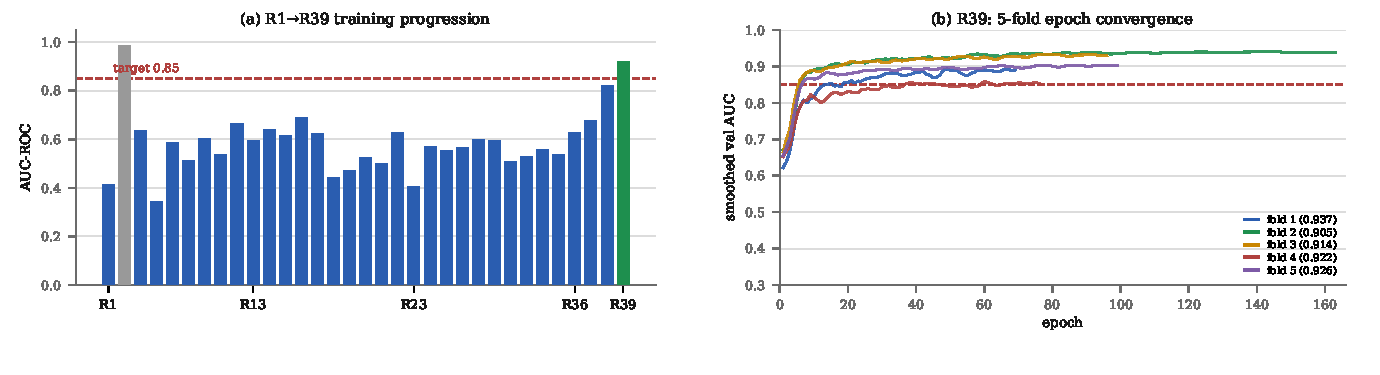
\includegraphics[width=\textwidth]{figures/fig_training_history.pdf}
\caption{(a) Mean and best AUC across all 39 tracked training runs, with R39
(749-model corpus) highlighted. (b) R39's five-fold validation-AUC
convergence, with final test AUC per fold in the legend.}
\label{fig:traininghistory}
\end{figure}

Table~\ref{tab:ablation} traces the three consecutive revisions on an earlier
238-model corpus that produced the largest single-run gains, because which
changes mattered is more instructive than the final number alone.

\begin{table}[h]
\centering
\caption{Three consecutive development runs producing the largest single-run
gains (238-model corpus revision; superseded by the 749-model results in
Table~\ref{tab:phase1}).}
\label{tab:ablation}
\small
\begin{tabularx}{\textwidth}{@{}L{1.6cm}XC{2.6cm}@{}}
\toprule
\textbf{Run} & \textbf{Change} & \textbf{Mean AUC} \\
\midrule
R35 & Populated previously dead hole-count / joint-type features & 0.539 \\
R36 & + spatial link signal, real contact-area edge weight & 0.628 (+0.089) \\
R37 & + negative-ratio $0.5\!\to\!1.0$ fix, promotion-gate fix, seeded splits & 0.677 (+0.049) \\
\bottomrule
\end{tabularx}
\end{table}

The single largest jump --- R35 to R36, at $+0.089$ mean AUC --- followed
directly from discovering that two node and edge features, hole count and
joint type, had been silently zero-valued since the project's inception. They
were being sourced from a file path that had never existed. Once populated
with real values, and paired with the spatial link signal from
Equation~\ref{eq:linkscore} and a genuine rather than hardcoded contact-area
edge weight, the encoder gained access to information it had never actually
had.

The second-largest gain, R36 to R37 at $+0.049$, came from correcting the
negative-sampling ratio described in Section~\ref{sec:metrics}, alongside
fixing the promotion-gate bug.

The pattern across both is worth stating plainly, because it runs against
expectation: \textbf{neither gain came from architecture search or
hyperparameter tuning}. Both came from correcting silently broken inputs to
metrics. The largest remaining improvement, from roughly 0.68 to 0.92, came
from replacing the corpus itself --- a data intervention, not a modelling
one.

\section{Phase 2: Next-Component Recommendation}
\label{sec:results-phase2}

NodeRanker achieves Hit@1 of 0.4093 against a corpus-wide majority-class
baseline of 0.3442. This is a genuine, non-trivial improvement over always
predicting the plurality class, and it is worth noting that earlier corpus
revisions produced a head that tied the baseline exactly --- a failure mode
that took several attempts to move past. Hit@5 reaches 0.9101, MRR 0.6102,
and NDCG@5 0.6754.

\begin{table}[h]
\centering
\caption{Phase 2 ranking metrics against the majority-class baseline.}
\label{tab:phase2}
\small
\begin{tabularx}{\textwidth}{@{}L{4.6cm}C{3.0cm}C{3.0cm}X@{}}
\toprule
\textbf{Metric} & \textbf{Validation} & \textbf{Test} & \textbf{Baseline} \\
\midrule
Hit@1   & 0.4188 & 0.4093 & 0.3442 \\
Hit@5   & 0.8885 & 0.9101 & --- \\
MRR     & 0.6041 & 0.6102 & --- \\
NDCG@5  & 0.6621 & 0.6754 & --- \\
\bottomrule
\end{tabularx}
\end{table}

The aggregate figure conceals a real weakness, and Table~\ref{tab:perclass}
exposes it.

\begin{table}[h]
\centering
\caption{NodeRanker per-class Hit@1 on the test split, with predicted versus
true class share.}
\label{tab:perclass}
\small
\begin{tabularx}{\textwidth}{@{}L{3.0cm}C{1.6cm}C{2.0cm}C{2.4cm}C{2.6cm}@{}}
\toprule
\textbf{Component type} & \textbf{$n$} & \textbf{Hit@1} & \textbf{True share} & \textbf{Predicted share} \\
\midrule
body         & 222 & 0.689 & 34.3\% & 53.1\% \\
nut          & 36  & 0.444 & 5.6\%  & 9.7\%  \\
thick\_plate & 111 & 0.360 & 17.1\% & 14.8\% \\
bolt         & 98  & 0.316 & 15.1\% & 12.0\% \\
long\_shaft  & 71  & 0.225 & 11.0\% & 5.6\%  \\
short\_shaft & 47  & 0.149 & 7.3\%  & 2.8\%  \\
thin\_plate  & 42  & 0.024 & 6.5\%  & 1.1\%  \\
washer       & 18  & 0.000 & 2.8\%  & 0.5\%  \\
\bottomrule
\end{tabularx}
\end{table}

Performance is markedly uneven. The majority class reaches 0.689 while
\texttt{washer} sits at exactly zero and \texttt{thin\_plate} at 0.024. The
head also over-predicts \texttt{body} relative to its true frequency, at
53.1\% of predictions against a 34.3\% true share.

This is a majority-class bias, and it is unresolved. It is reported here
rather than obscured behind the headline Hit@1 because the distinction
matters for anyone considering deploying the ranking head: the system is
substantially more reliable at recommending a housing than a washer, and a
user should know that. Section~\ref{sec:limitations} returns to it.

\section{Phase 3: Shape Generation}

HybridShapeGenerator reaches a test IoU of 0.6459 and Chamfer distance of
0.0377, against targets of IoU $\geq$ 0.35 and Chamfer $\leq$ 0.08. The
selected checkpoint recorded validation IoU 0.6640 and Chamfer 0.0359.

\begin{table}[h]
\centering
\caption{Phase 3 shape-generation metrics.}
\label{tab:phase3}
\small
\begin{tabularx}{\textwidth}{@{}L{4.6cm}C{2.8cm}C{2.8cm}X@{}}
\toprule
\textbf{Metric} & \textbf{Validation} & \textbf{Test} & \textbf{Target} \\
\midrule
IoU              & 0.6640 & 0.6459 & $\geq$ 0.35 \\
Chamfer distance & 0.0359 & 0.0377 & $\leq$ 0.08 \\
Total loss       & 0.2122 & 0.2234 & --- \\
\quad BCE term   & 0.0736 & 0.0749 & --- \\
\quad Dice term  & 0.2454 & 0.2670 & --- \\
\quad KL term    & 0.3191 & 0.2999 & --- \\
\bottomrule
\end{tabularx}
\end{table}

One result requires careful interpretation. Across all 285 test samples,
\emph{none} fell below the retrieval confidence threshold, so the VAE
fallback was never invoked during this evaluation run. It would be easy to
read that as evidence that the generative component is unnecessary. It is
not. It indicates that retrieval alone currently covers the test distribution
at the configured threshold --- a result specific to this corpus's category
coverage. A corpus containing more geometrically varied or less standardised
components would exercise the fallback, and the threshold analysis would need
re-running.

\section{Ablation Studies}
\label{sec:ablations}

Four controlled experiments were run to test design decisions that would
otherwise rest on assumption. Each is reported with its outcome, including the
two that did \emph{not} support the change being tested.

\subsection{Encoder Benchmark}

RGATConv was benchmarked against GATv2, GraphSAGE and GIN. Per-stage widths
were held constant across all four candidates, so the comparison isolates the
aggregation mechanism rather than confounding it with layer capacity. GraphSAGE
and GIN lose edge features entirely --- neither accepts an \texttt{edge\_dim}
--- which is a real asymmetry, and a deliberate one: part of what the benchmark
was meant to surface was whether the joint-type and contact-area edge features
are actually load-bearing.

\begin{table}[h]
\centering
\caption{Encoder benchmark. Two-fold screening against full five-fold validation.}
\label{tab:encoderbench}
\small
\begin{tabularx}{\textwidth}{@{}L{2.6cm}L{4.4cm}C{2.6cm}C{2.6cm}@{}}
\toprule
\textbf{Encoder} & \textbf{Edge features used} & \textbf{2-fold screen} & \textbf{Full 5-fold} \\
\midrule
RGATConv & Joint type + contact area & lower & \textbf{0.6765} \\
GraphSAGE & None & apparently higher & 0.6717 \\
GATv2 & Contact area (layer 1) & --- & --- \\
GIN & None & --- & --- \\
\bottomrule
\end{tabularx}
\end{table}

The result is worth recording precisely because it is a near-miss. Two-fold
screening suggested GraphSAGE was ahead, and acting on that screen would have
removed relational attention from the architecture. Full five-fold validation
showed an essential tie --- 0.6765 against 0.6717, well inside the fold-to-fold
spread. RGATConv was retained.

The methodological lesson generalises: an under-powered screening protocol does
not merely produce a noisy estimate, it can invert the ranking of two
candidates and drive a permanent architectural decision the wrong way.

\subsection{Capacity Ablation}

Two capacity parameters were varied against the then-current baseline of 0.6765
mean AUC.

\begin{table}[h]
\centering
\caption{Capacity ablation outcomes.}
\label{tab:capacity}
\small
\begin{tabularx}{\textwidth}{@{}L{4.0cm}C{3.0cm}X@{}}
\toprule
\textbf{Change} & \textbf{Mean AUC} & \textbf{Outcome} \\
\midrule
Baseline (dropout 0.2) & 0.6765 & Reference \\
Dropout $\to$ 0.3 & \textbf{0.6875} & Promoted; retained in the final configuration \\
Hidden dim $\to$ 256 & --- & Hard MPS out-of-memory crash; not evaluable on this hardware \\
\bottomrule
\end{tabularx}
\end{table}

Raising dropout to 0.3 produced a modest but real gain at full five-fold rigour
and was promoted. Widening the hidden dimension to 256 could not be assessed at
all: it exceeds the Metal Performance Shaders allocation ceiling of the
development machine. That is a hardware limit rather than a negative result,
and it is recorded as such rather than as evidence that wider is not better.

\subsection{Learning Curve}

To establish whether the system was data-limited or model-limited, Phase~1 was
retrained on nested subsets of the corpus.

\begin{table}[h]
\centering
\caption{Phase 1 performance against training-corpus fraction.}
\label{tab:learningcurve}
\small
\begin{tabularx}{\textwidth}{@{}C{4.0cm}C{4.0cm}X@{}}
\toprule
\textbf{Corpus fraction} & \textbf{Mean AUC} & \textbf{Trend} \\
\midrule
25\%  & 0.5736 & --- \\
50\%  & intermediate & rising \\
75\%  & intermediate & rising \\
100\% & 0.6627 & no plateau observed \\
\bottomrule
\end{tabularx}
\end{table}

Performance scales cleanly with corpus size across the full range, with no sign
of saturation at 100\%. The system was therefore \emph{data-limited} at that
point, not architecture-limited --- which directly motivated the corpus
expansion from 238 to 749 models described in Section~\ref{sec:corpus}, and
predicted the large gain that expansion subsequently produced.

\subsection{Cross-Validation Protocol}

An early protocol used a fixed test set reused across all five folds. It was
replaced with true five-fold assignment, in which each fold rotates a genuinely
independent test partition.

\begin{table}[h]
\centering
\caption{Fixed test set versus true five-fold assignment, same corpus.}
\label{tab:cvprotocol}
\small
\begin{tabularx}{\textwidth}{@{}L{5.0cm}C{3.4cm}X@{}}
\toprule
\textbf{Protocol} & \textbf{Mean AUC} & \textbf{Std} \\
\midrule
Fixed test set, reused $\times$5 & 0.6875 & $\pm$0.0274 \\
True five-fold assignment & 0.6937 & $\pm$0.0702 \\
\bottomrule
\end{tabularx}
\end{table}

The means are essentially identical; the standard deviation is roughly two and
a half times larger under the honest protocol. The fixed test set had not been
\emph{inflating} the reported mean --- it had been \emph{masking} genuine
fold-to-fold variance. Every Phase~1 number reported in this chapter uses the
true five-fold protocol.

\subsection{Part Bank Quality Gate}

The retrieval bank was rebuilt with a geometric quality gate applied at
indexing time, rejecting degenerate and malformed bodies.

\begin{table}[h]
\centering
\caption{Part bank composition before and after the quality gate.}
\label{tab:partbank}
\small
\begin{tabularx}{\textwidth}{@{}L{4.6cm}C{3.0cm}C{3.0cm}X@{}}
\toprule
\textbf{Bank version} & \textbf{Parts} & \textbf{Assemblies} \\
\midrule
No gate & 4{,}500 & 187 \\
With quality gate & 3{,}843 & 193 \\
\bottomrule
\end{tabularx}
\end{table}

The gate removed roughly 15\% of indexed parts while \emph{increasing} the
number of contributing assemblies, which is the expected signature of
eliminating many degenerate fragments drawn from a few pathological files.
Comparing the two rebuilds also surfaced a signed-versus-absolute volume bug
that had been silently admitting inverted-normal bodies into the bank.

\section{Findings from Exploratory Data Analysis}
\label{sec:eda-finding}

A full exploratory pass over the final 648-graph corpus, run \emph{after}
model training had already completed successfully, surfaced a data-quality
issue invisible to the training metrics themselves.

The SDF-mean node feature is exactly zero for 25,142 of 25,155 bodies ---
99.95\% of the entire corpus. Only 13 bodies carry a non-zero value, and the
paired SDF-variance feature moves in near-perfect lockstep with it (Pearson
$r > 0.999$), which is consistent with a feature that is silently constant
rather than genuinely near-zero for physically flat geometry.

This mirrors the earlier instance described in Section~\ref{sec:devhistory},
where hole-count and joint-type features were found to have been dead since
the project's inception. That earlier discovery produced the single largest
one-run performance gain of the entire project.

The finding is reported here unresolved, rather than omitted, because it
demonstrates something worth stating: a model reaching strong aggregate
metrics is not sufficient evidence that every input feature is contributing.
A 34-dimensional feature vector of which one pair is constant still trained
to 0.92 AUC. Targeted exploratory analysis of the corpus remains necessary
even after training succeeds, and is recommended here as standard practice
for any comparable pipeline.

A second, related finding emerged from the same analysis. Some 72.1\% of
bolts and 83.5\% of washers in the corpus are flagged by the geometric hole
detector as having holes --- a higher rate than \texttt{thick\_plate} bodies
at 47.8\%, which structurally host the through-holes that fasteners actually
sit in. A washer's own bore is a genuine hole, so a high rate there is
expected; a solid bolt normally is not. The elevated rate plausibly reflects
the detector picking up thread-groove or head-recess geometry as false
positives on a meaningful fraction of bolts. This is flagged as a candidate
data-quality issue for future correction rather than a confirmed bug, since
it has not yet been manually verified against individual STEP files at scale.

\section{Discussion}

Three observations stand out from the results as a whole.

\textbf{Data quality dominated architecture.} The two largest single-run
gains in a thirty-nine-revision history both came from repairing silently
broken inputs, and the largest improvement overall came from replacing the
corpus. No architecture search or hyperparameter sweep in this project
produced a comparable effect. For a project of this scale on a modest corpus,
effort spent auditing inputs returned considerably more than effort spent
searching model space.

\textbf{Aggregate metrics conceal structure.} Phase~2's Hit@1 of 0.4093
genuinely exceeds baseline, and simultaneously conceals a head that cannot
identify a washer at all. Reporting per-class breakdowns alongside aggregates
is not a courtesy; without Table~\ref{tab:perclass} the Phase~2 result would
be actively misleading.

\textbf{Retrieval-first was the right default for this domain.} Industrial
fasteners are highly standardised, and a part bank holding hundreds of real
examples will usually contain something closer to correct than a
$32^3$-resolution generative sample. The architecture reflects a judgement
about the domain rather than about model capability.

%% =====================================================================
\chapter{Application Interface and Demonstration}
\label{ch:ui}
%% =====================================================================

This chapter documents the deployed application through screenshots of the
running system, captured on 18~September 2026. The application is the
Streamlit front end described in Section~\ref{sec:explainlayer}: a single
page with a control sidebar and a dual-panel workspace, in which a user
uploads a STEP file and receives the detected, ranked, generated and explained
results without leaving the page. The demonstration asset is a tool-post
assembly, derived from the corpus model \texttt{Tool\_Post\_10}, from which
fasteners, springs, shafts and the knob were deliberately removed so that the
correct answer is known (Section~\ref{sec:ui-reconstruct}).

%% ---------------------------------------------------------------------
\section{Application Overview}
%% ---------------------------------------------------------------------

Figure~\ref{fig:ui-overview} shows the application in its initial state,
before any file is loaded. The window has three regions. The \emph{sidebar}
on the left carries the viewer settings, the trained-model information and
the activity log. The \emph{workspace} occupies the centre and is divided into
an \emph{Input} panel and a \emph{Results} panel. The \emph{AIDA panel} below
the workspace stays empty until inference finishes, and then holds the
engineering-language explanation of the predictions.

\begin{figure}[H]
\centering
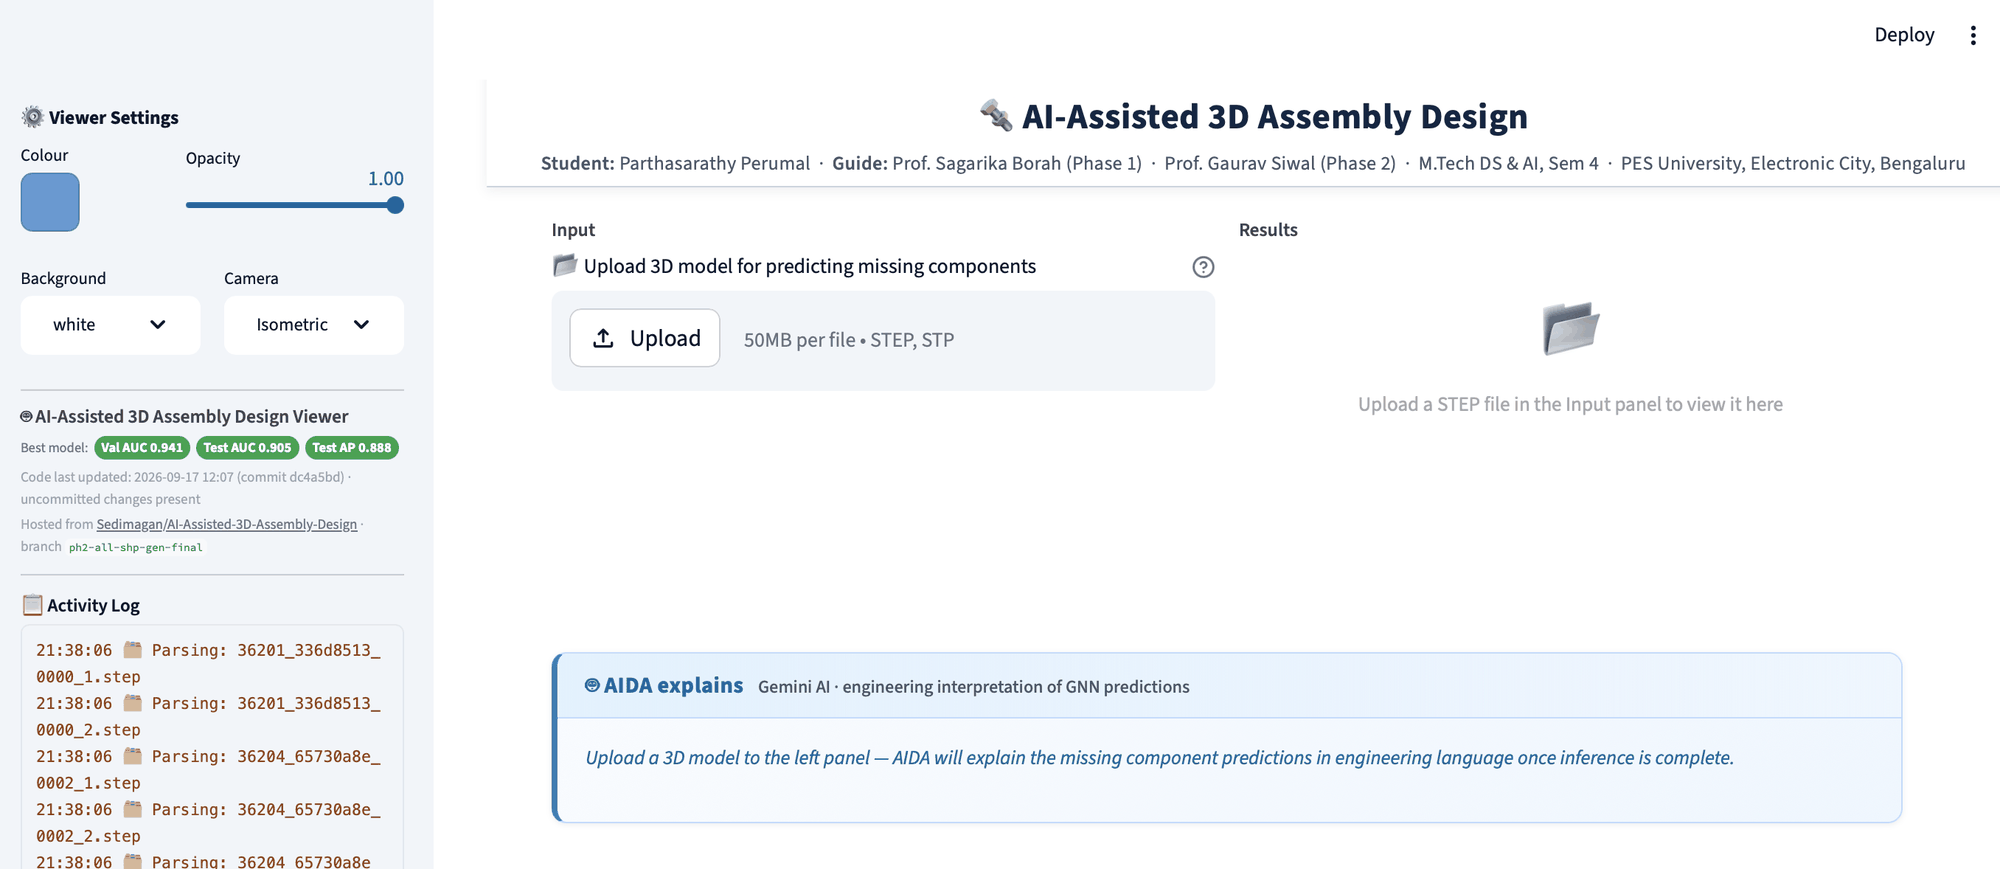
\includegraphics[width=\textwidth]{figures/ui_full_view.png}
\caption{Full application window in its initial state: sidebar (left), Input
and Results panels (centre) and the AIDA explanation panel (bottom).}
\label{fig:ui-overview}
\end{figure}

%% ---------------------------------------------------------------------
\section{Sidebar Controls}
%% ---------------------------------------------------------------------

\subsection{Viewer Settings}

The viewer settings, shown in Figure~\ref{fig:ui-viewer}, control how the 3D
model is drawn and do not affect any prediction. \emph{Colour} sets the base
colour of the assembled parts, \emph{Opacity} ranges from 0.10 to 1.00 so that
internal components such as balls and springs can be seen through their
housings, \emph{Background} sets the scene background (white in the figure),
and \emph{Camera} selects the viewing preset (isometric in the figure).

\begin{figure}[H]
\centering
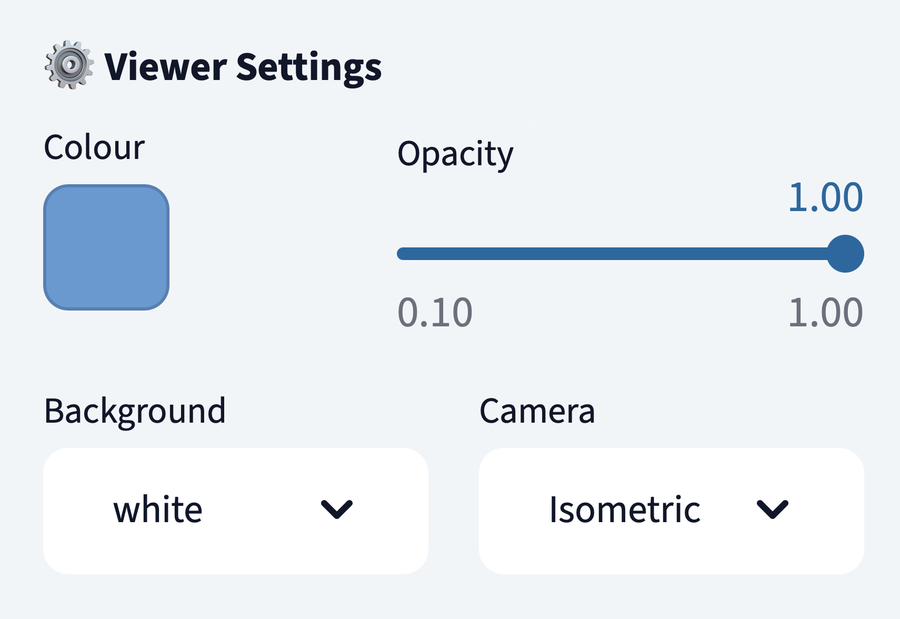
\includegraphics[width=0.5\textwidth]{figures/ui_viewer_settings.png}
\caption{Viewer Settings: part colour, opacity, background and camera preset.}
\label{fig:ui-viewer}
\end{figure}

\subsection{Trained-Model Information}

The sidebar reports which model is currently serving predictions
(Figure~\ref{fig:ui-model}). Three badges give the validation AUC-ROC (0.941),
the test AUC-ROC (0.905) and the test average precision (0.888) recorded for
the promoted checkpoint; a badge is green when its AUC is at least 0.70. These
are single-checkpoint figures and differ from the five-fold means of
Table~\ref{tab:phase1}, which are the results this project reports. Beneath the
badges the application shows the date and commit of the code it is running,
whether uncommitted changes are present, and the repository and branch it was
served from, so that any screenshot can be traced to a specific code state.

\begin{figure}[H]
\centering
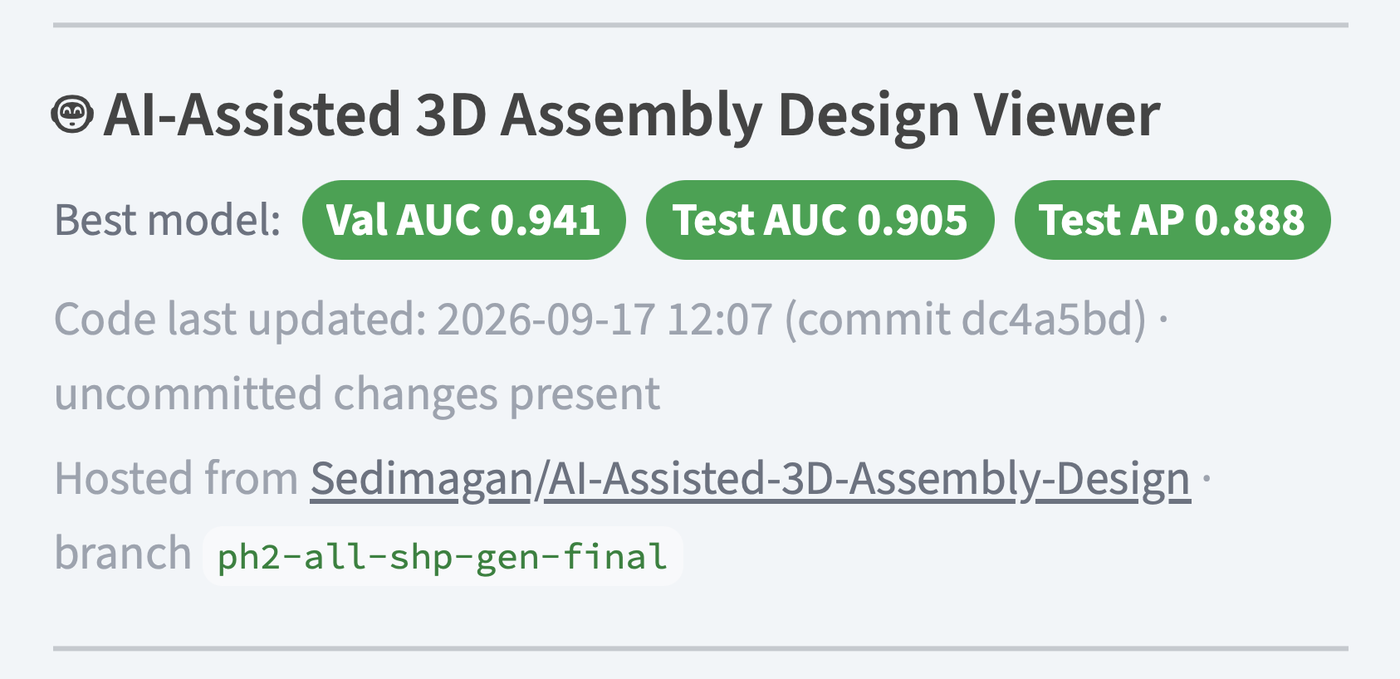
\includegraphics[width=0.85\textwidth]{figures/ui_model_info.png}
\caption{Trained-model information: metrics of the promoted serving
checkpoint and the code version the application is running.}
\label{fig:ui-model}
\end{figure}

\subsection{Activity Log}

The activity log (Figure~\ref{fig:ui-log}) records each pipeline stage with a
timestamp as it runs: STEP files being parsed, the assembly graphs built and
saved, the split summary, and the stage markers of the inference run, for
example \texttt{[2/4] Building model}. It makes the multi-second processing
time visible to the user and is the first place to look when a stage fails.
A \emph{Reset All \& Log} control (Figure~\ref{fig:ui-details}) clears it.

\begin{figure}[H]
\centering
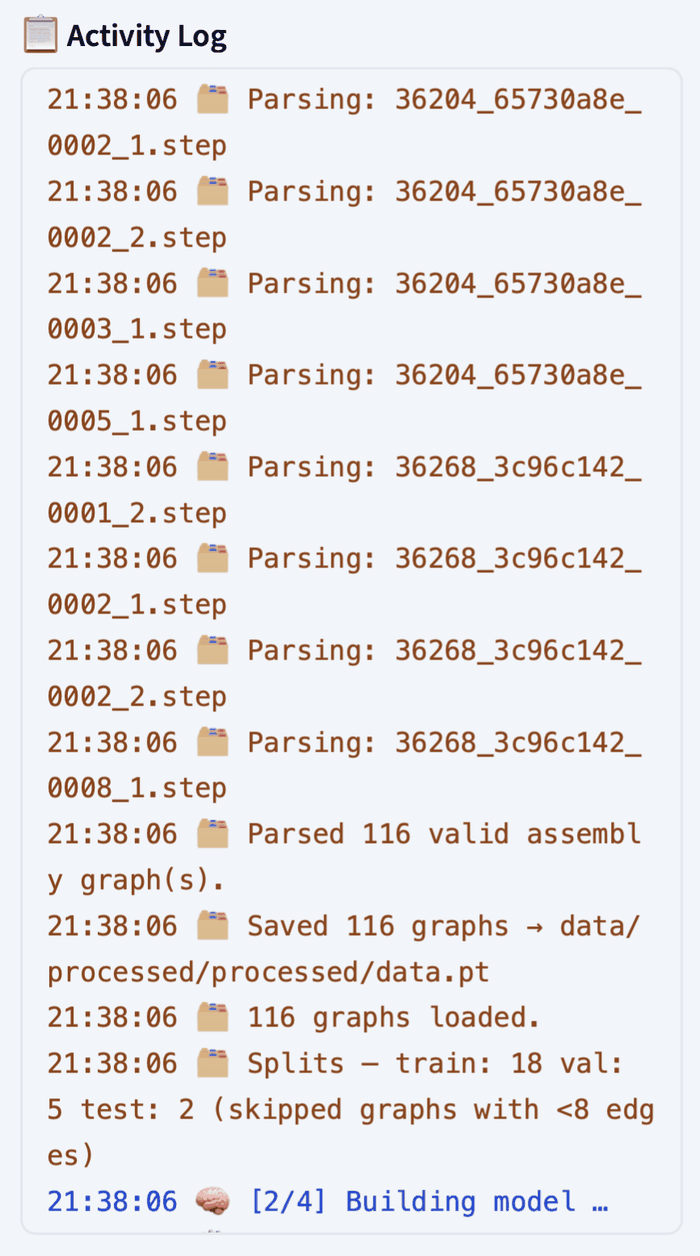
\includegraphics[width=0.4\textwidth]{figures/ui_activity_log.png}
\caption{Activity Log: timestamped pipeline stages.}
\label{fig:ui-log}
\end{figure}

%% ---------------------------------------------------------------------
\section{Input and Results Panels}
%% ---------------------------------------------------------------------

\subsection{Model Upload}

The Input panel accepts a single STEP or STP file of up to 50~MB through the
upload control shown in Figure~\ref{fig:ui-input}(a). Until a file is loaded,
the Results panel displays a prompt asking for one
(Figure~\ref{fig:ui-input}(b)).

\begin{figure}[H]
\centering
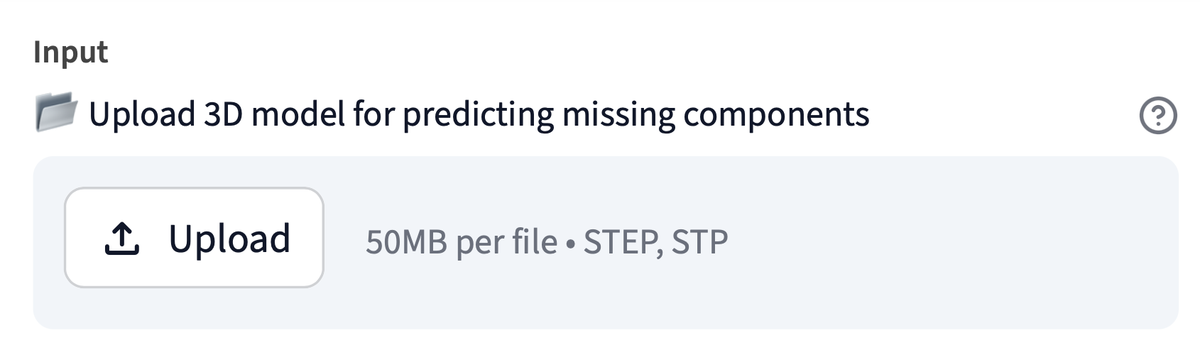
\includegraphics[width=0.8\textwidth]{figures/ui_input_panel.png}\\[8pt]
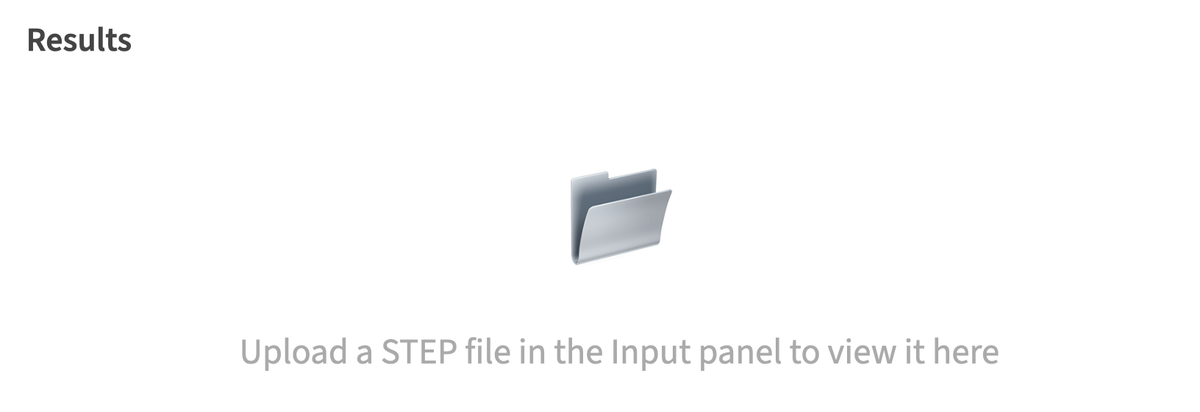
\includegraphics[width=0.8\textwidth]{figures/ui_results_empty.png}
\caption{(a)~Input panel with the STEP/STP upload control. (b)~Results panel
before a file is loaded.}
\label{fig:ui-input}
\end{figure}

\subsection{Inspecting the Uploaded Assembly}

Once a file is parsed, the Results panel shows the model in an interactive 3D
viewer (Figure~\ref{fig:ui-before}). A \emph{Original}/\emph{Result} toggle
switches between the uploaded geometry and the prediction overlay, and
\emph{Highlight} toggles emphasis on the selected component. Each body appears
as a separately switchable entry in the legend (\emph{Part~1} to \emph{Part~4}
here), and the toolbar provides screenshot capture, zoom, pan, orbit, turntable
rotation, home view, camera reset and full-screen mode. The model can be
inspected from any angle before any prediction is run, which is how a user
confirms that the file loaded as intended.

\begin{figure}[H]
\centering
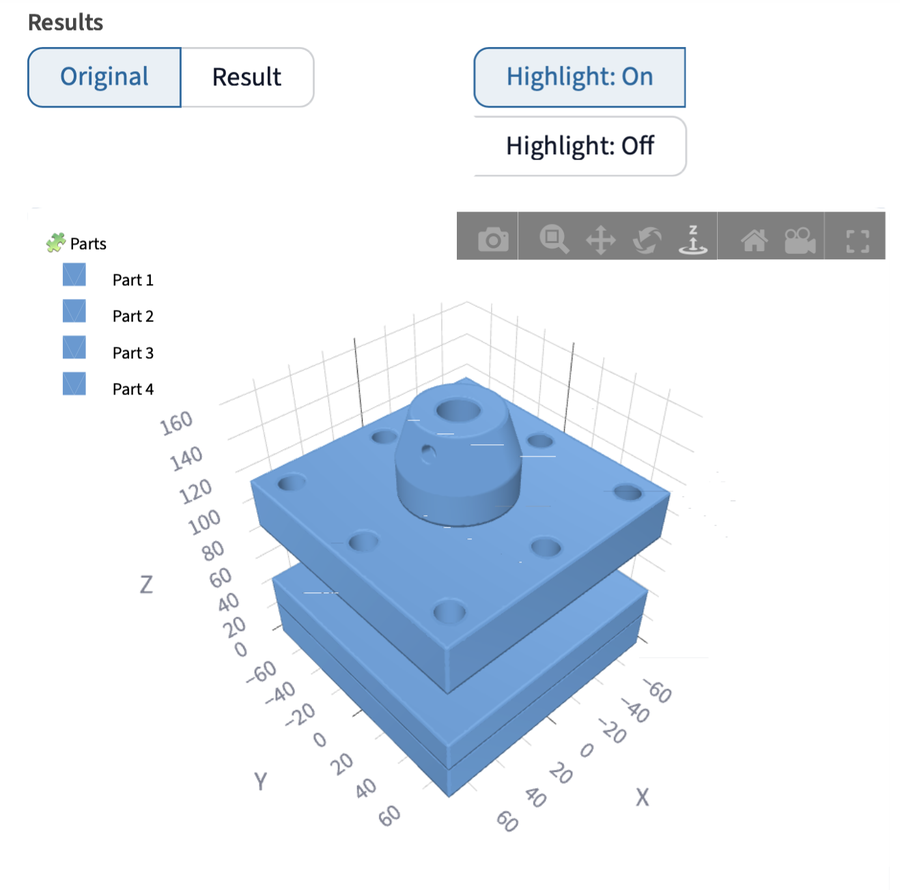
\includegraphics[width=0.6\textwidth]{figures/ui_view_before.png}
\caption{Original view of the uploaded partial tool-post assembly, before
prediction.}
\label{fig:ui-before}
\end{figure}

%% ---------------------------------------------------------------------
\section{Prediction Results}
%% ---------------------------------------------------------------------

\subsection{Result View}

Selecting \emph{Result} overlays the predictions on the uploaded model
(Figure~\ref{fig:ui-suggested}). Components are grouped in the legend by their
status. \emph{Parts} (blue) are components with their expected contacts.
\emph{Not Assembled} (orange, marked with a warning symbol) are components
flagged either because they touch nothing or because they have fewer contacts
than other instances of the same part. \emph{Suggested Shapes} (pink) are the
geometries proposed for the missing components. Each group can be shown or
hidden individually, and the row of buttons beneath the viewer switches whole
groups on or off at once. The caption line under the viewer reports the file
name and the mesh size that was processed (here 76,996 points and 154,008
faces).

\begin{figure}[H]
\centering
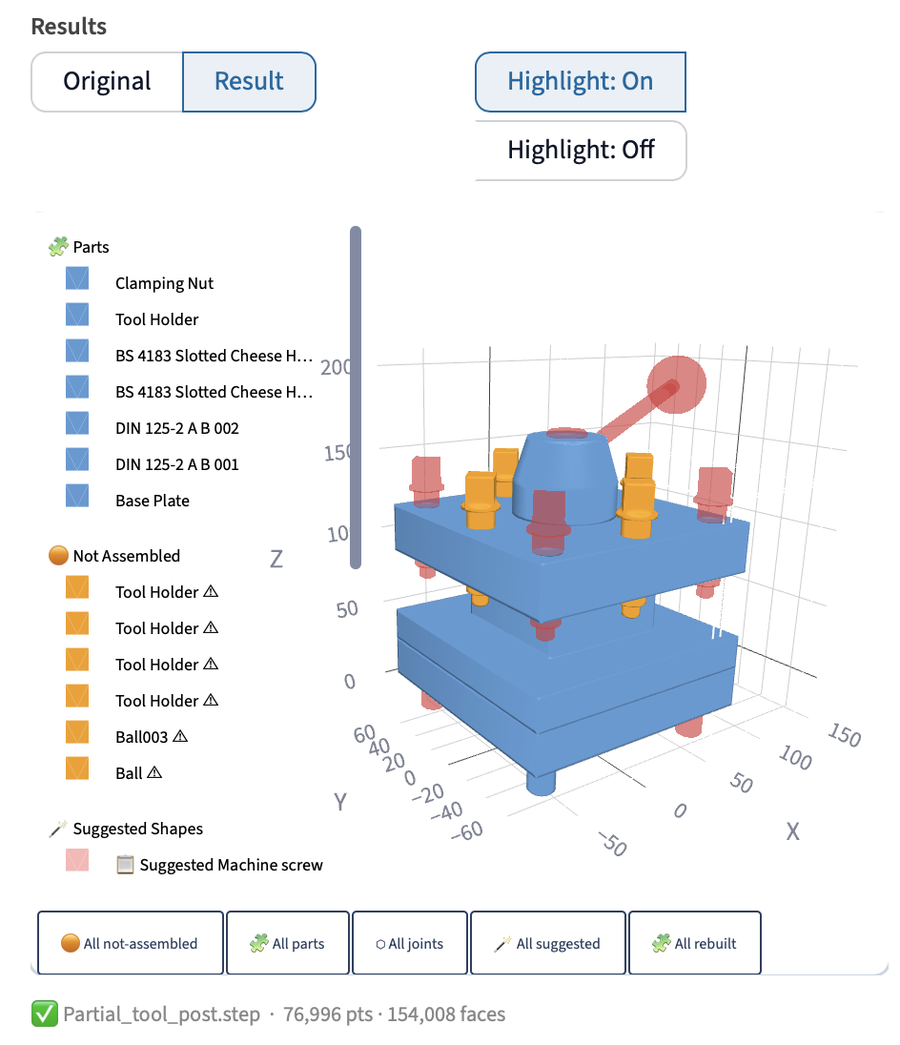
\includegraphics[width=0.6\textwidth]{figures/ui_view_suggested.png}
\caption{Result view of the partial tool post: Parts (blue), Not Assembled
(orange) and the Suggested Shapes group (pink).}
\label{fig:ui-suggested}
\end{figure}

\subsection{Reconstructed Components}
\label{sec:ui-reconstruct}

For tool-post assemblies the application additionally reconstructs the missing
components and draws them in a separate \emph{Reconstructed} group, coloured by
component category so that fasteners, springs, shafts and the knob can be told
apart (Figure~\ref{fig:ui-reconstructed}). The step is implemented in
\texttt{slot\_detector.py} and \texttt{rebuild.py}, and works in three stages.
First, it locates \emph{open seats}: cylindrical holes on the host bodies with
nothing seated in them, plus positions implied by the rotational symmetry of a
hole pattern that has surviving members. Second, it assigns each seat a
component family from the seat geometry and the parts around it. Third, it
obtains the geometry. Where an identical part survives elsewhere in the upload,
its mesh is copied and translated to the empty seat. Otherwise the part is
retrieved from the part bank or from a small library of springs, which the
bank's watertightness gate cannot hold, using the corpus assemblies most
similar to the upload to choose between candidates. The components in
Figure~\ref{fig:ui-reconstructed} are in the same positions as the suggested
shapes of Figure~\ref{fig:ui-suggested}, drawn under the category colouring
instead.

\begin{figure}[H]
\centering
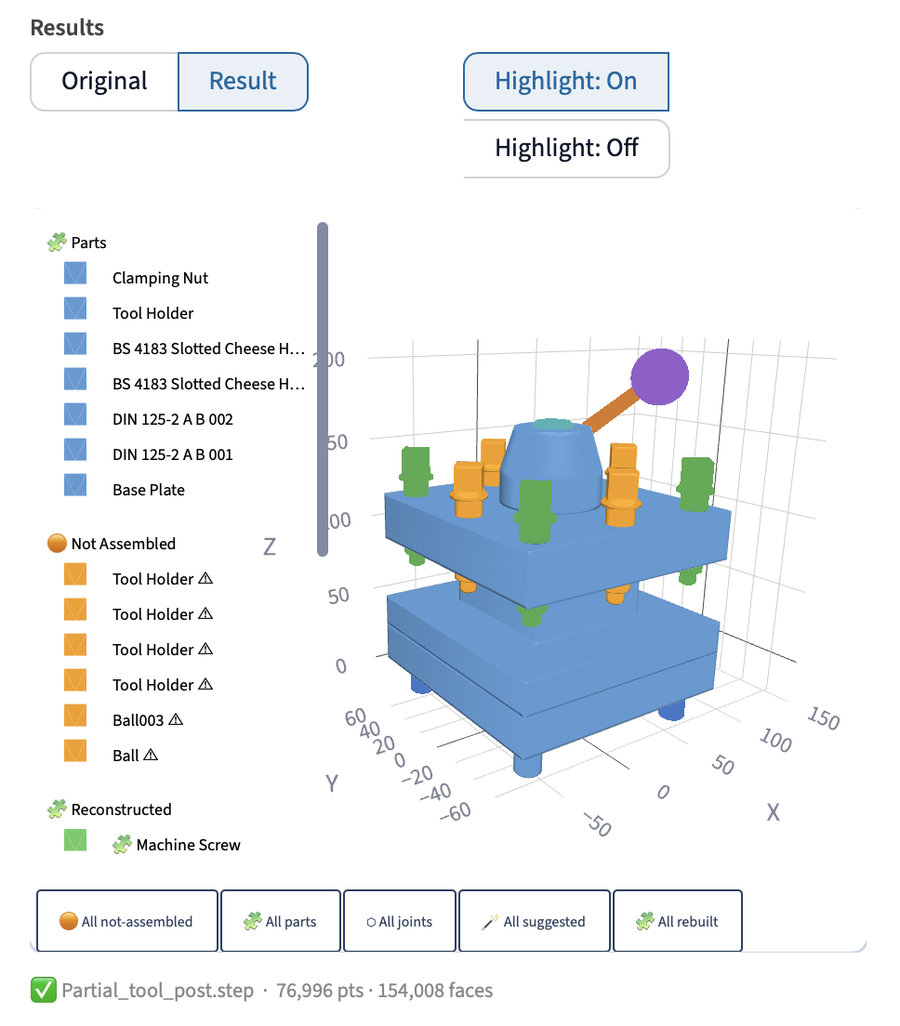
\includegraphics[width=0.6\textwidth]{figures/ui_view_reconstructed.png}
\caption{The same components in the Reconstructed group, coloured by
component category.}
\label{fig:ui-reconstructed}
\end{figure}


The reconstruction was scored against the withheld original. Table~\ref{tab:recon}
reports, for each component family, the distance between the rebuilt part's
centroid and the matching part in the original assembly (position), and the
mean surface distance between the two meshes after centring both (shape and
orientation). Across the 17 rebuilt components the mean position error is
0.27~mm and the mean shape error is 0.39~mm. Re-running with the original
model's own parts excluded from retrieval gives the same figures. Two
independent tessellations of the \emph{same} solid differ by roughly
0.2--0.6~mm, so shape errors inside that band are indistinguishable from an
exact match. The central shaft (0.83~mm) is the only family above it, and the
knob has the largest position error (2.93~mm).

\begin{table}[H]
\centering
\caption{Reconstruction accuracy against the original \texttt{Tool\_Post\_10}
(17 components; mean per family, in mm).}
\label{tab:recon}
\small
\begin{tabularx}{\textwidth}{@{}L{3.3cm}C{0.9cm}L{5.5cm}C{1.9cm}C{1.9cm}@{}}
\toprule
\textbf{Family} & \textbf{n} & \textbf{Geometry source} & \textbf{Position} & \textbf{Shape} \\
\midrule
Machine screw      & 4 & Copied from surviving instance & 0.00 & 0.41 \\
BS~4183 screw      & 2 & Copied from surviving instance & 0.00 & 0.49 \\
DIN washer         & 2 & Copied from surviving instance & 0.00 & 0.29 \\
Ball               & 2 & Copied from surviving instance & 0.00 & 0.10 \\
Compression spring & 4 & Retrieved (spring library)     & 0.07 & 0.36 \\
Central shaft      & 1 & Retrieved (part bank)          & 0.32 & 0.83 \\
Side shaft         & 1 & Retrieved (part bank)          & 1.14 & 0.45 \\
Knob               & 1 & Retrieved (part bank)          & 2.93 & 0.54 \\
\midrule
\textbf{All}       & \textbf{17} & & \textbf{0.27} & \textbf{0.39} \\
\bottomrule
\end{tabularx}
\end{table}

This result should be read narrowly. It is one assembly. The family rules and
the mount-hole rule for the side shaft are calibrated for the tool-post
category, and that same model was used to tune them, so the table demonstrates
that the mechanism can recover a known answer rather than establishing how it
generalises to unseen assemblies or other categories. The exclusion test
removes the original's parts from retrieval but does not remove the model from
the calibration. A held-out evaluation on further partial tool posts, and an
equivalent calibration for the other six categories, remain to be done.

\subsection{Prediction Details Panel}

When inference completes, a green banner reports how many missing components
were reconstructed and placed (Figure~\ref{fig:ui-details}). The reconstructed
components can be expanded into a table giving each component's position, how
its seat was found, where its shape came from, and the part used, and the
result can be downloaded as a \texttt{.glb} file for use in other 3D tools.
Below the reconstruction sits a summary line (here four components and six
known connections) and six collapsible sections: \emph{Assembly Type
Identified}, \emph{Expected Components Missing} (the
AssemblyTemplateDB prior), \emph{AI-Ranked Next Component} (the NodeRanker
output), \emph{Why This Next Component?} (the GNNExplainer attributions),
\emph{Open Assembly Joints Detected} (the octree open-surface findings) and
\emph{Suggested Missing-Part Shapes}. \emph{Predict another} loads a new file,
and \emph{Reset All \& Log} clears the session.

\begin{figure}[H]
\centering
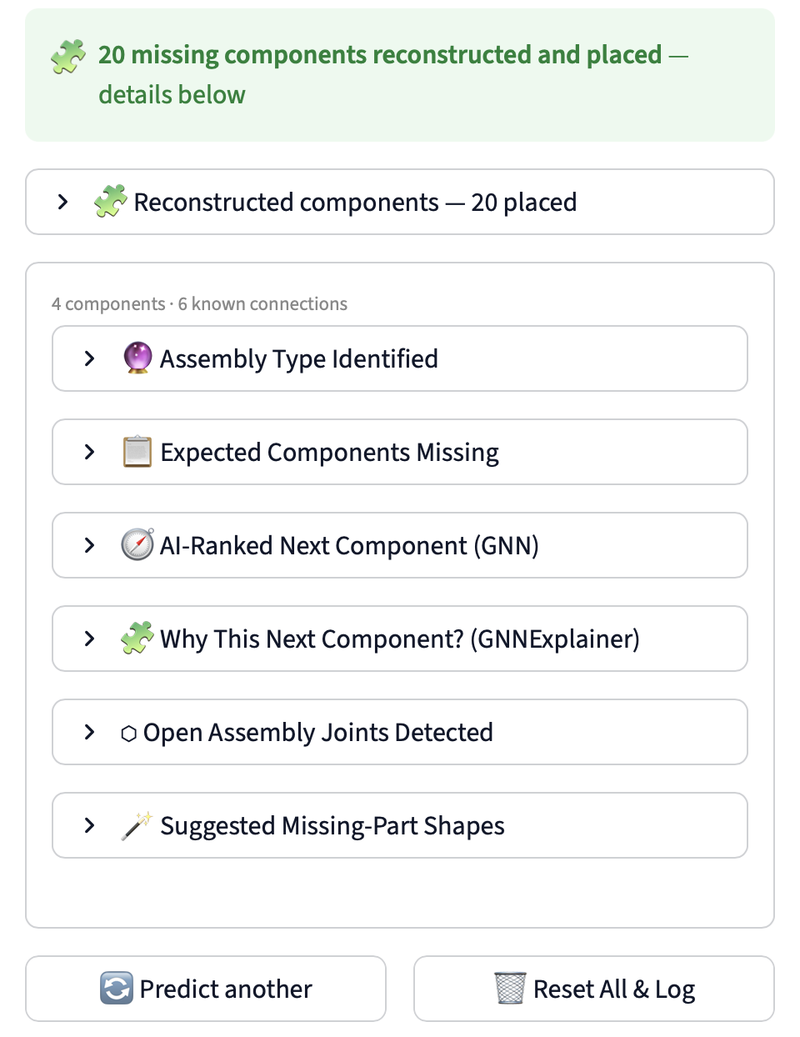
\includegraphics[width=0.5\textwidth]{figures/ui_output_details.png}
\caption{Prediction details panel with the reconstruction banner and the six
result sections.}
\label{fig:ui-details}
\end{figure}

%% ---------------------------------------------------------------------
\section{AIDA Engineering Interpretation}
%% ---------------------------------------------------------------------

The AIDA panel (Figure~\ref{fig:ui-aida}) turns the model outputs into an
engineering-language report with fixed sections. Section~1 lists components
that touch nothing, or that have fewer contacts than sibling instances of the
same part; in this run none met either condition. Section~2 lists the links
the GNN predicts between existing parts. Here every one carries a confidence
of 0.001, and AIDA reports them as very low confidence rather than presenting
them as findings. Section~3 reports the octree detector's open-surface
fractions (34\%, 30\% and 29\% for Bodies~2, 3 and~4). Section~4 lists the
suggested missing-part shapes together with a location fit and a shape
confidence for each: the washer, nut and bolt are retrieved from the part bank
at 99--100\% on both scores, while the long shaft is generated by the
conditional VAE with a 97\% shape confidence but only 34\% location fit. The
last item is worth noting. It shows the VAE fallback being used for a
non-fastener type in the live application, and it shows that for the generated
part the weak point is the placement, not the shape. A closing recommendation
summarises the findings.

\begin{figure}[H]
\centering
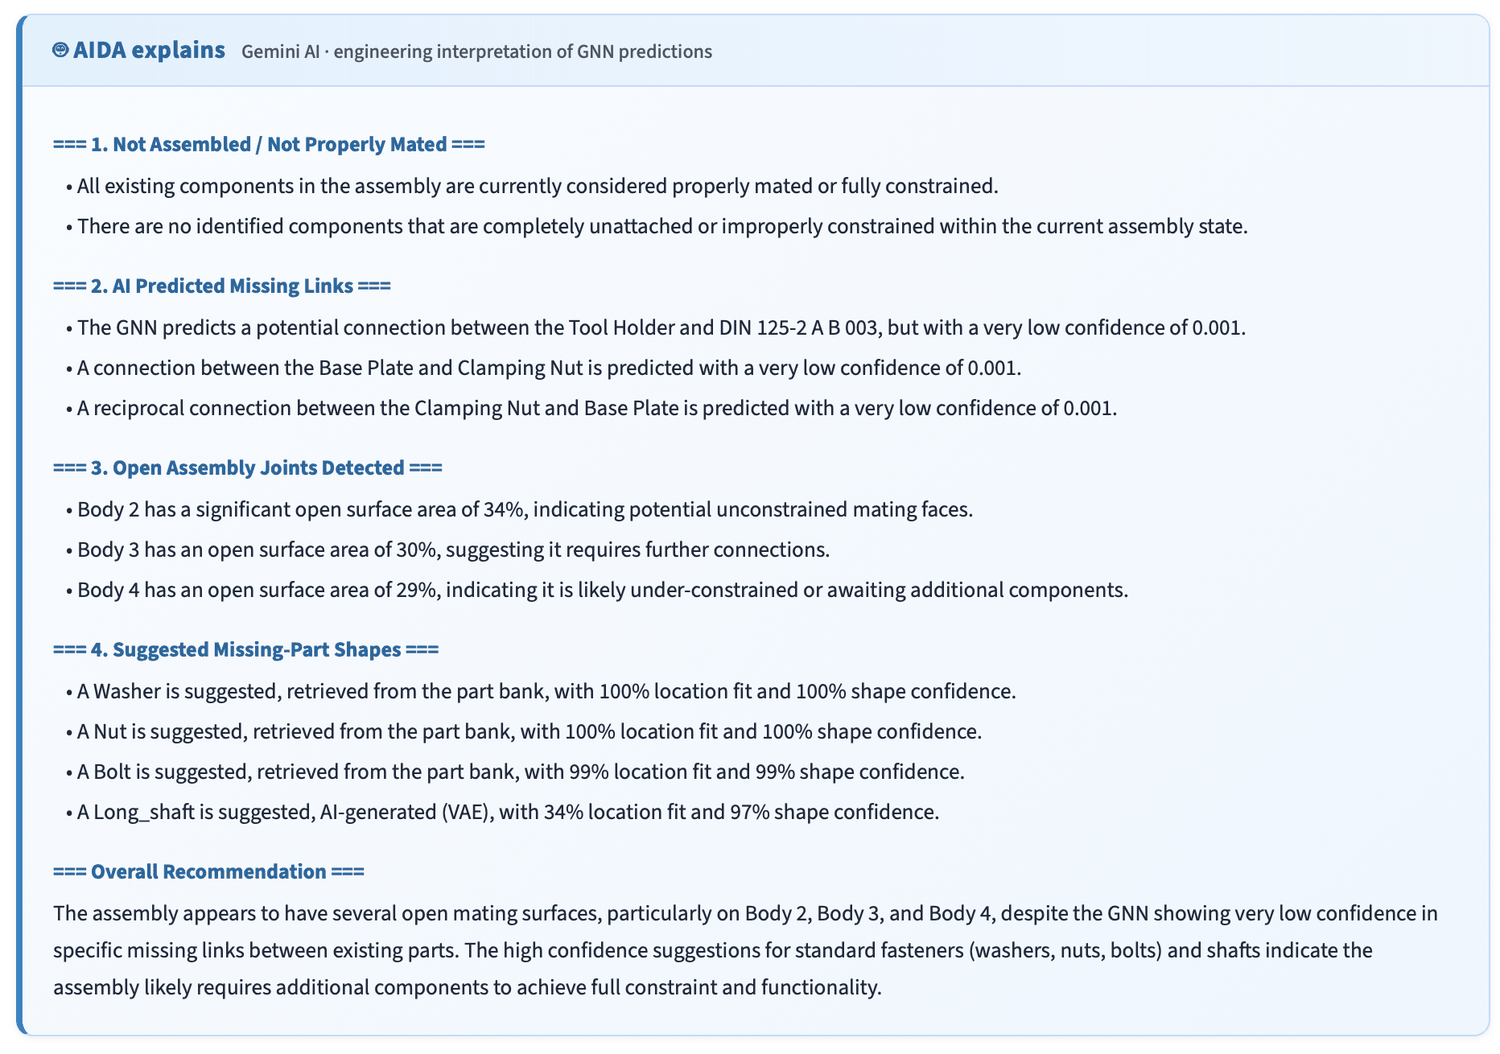
\includegraphics[width=0.95\textwidth]{figures/ui_aida.png}
\caption{AIDA panel: Gemini-generated engineering interpretation of the GNN
predictions, open-surface findings and suggested shapes.}
\label{fig:ui-aida}
\end{figure}

%% =====================================================================
\chapter{Testing and Validation}

This chapter describes how the system's correctness was established, separately
from how its performance was measured. The distinction matters: a model can
post a strong AUC while a defect upstream of it quietly corrupts the inputs, as
Section~\ref{sec:eda-finding} demonstrates.

\section{Reproducibility Protocol}

Every reported metric must be reproducible from the same corpus snapshot. This
was not true early in the project, and making it true required fixing a real
defect.

\texttt{get\_splits()} seeds the per-graph edge split, but it originally seeded
only the PyTorch generator and not Python's own. Because \texttt{RandomLinkSplit}
draws on both, re-evaluating an identical checkpoint on an identical fold
produced a slightly different AUC on each run. The fix seeds both generators
per \emph{(fold, graph)} pair. Verification was direct: the same checkpoint,
re-evaluated on the same fold, now returns a bit-identical AUC.

\begin{table}[h]
\centering
\caption{Reproducibility controls.}
\label{tab:repro}
\small
\begin{tabularx}{\textwidth}{@{}L{4.4cm}X@{}}
\toprule
\textbf{Control} & \textbf{Mechanism} \\
\midrule
Split determinism & Both RNGs seeded per (fold, graph) in \texttt{get\_splits()} \\
Feature-set versioning & Cache invalidated whenever the node-vector width changes \\
Configuration capture & Every checkpoint stores the \texttt{config.yaml} it trained under \\
Metric provenance & Checkpoints embed their own CV summary and test metrics \\
Batch determinism & Sampler shuffle seeded from the resumed epoch, not a reset counter \\
\bottomrule
\end{tabularx}
\end{table}

The feature-set versioning control deserves a note, because it was added after
a near-miss. The per-graph cache is keyed by filename alone. When the node
vector grew from 22 to 34 dimensions, 235 graphs cached under the old width
were about to be silently mixed into a dataset built under the new one,
producing a corpus of inconsistent tensor widths. A version stamp on the
feature set now invalidates the cache whenever the vector changes.

\section{Validation of the Graph Construction Pipeline}

The pipeline is validated at three levels.

\textbf{Structural validation.} Every parsed graph is checked for node/edge
count consistency, correct feature-vector width, and absence of self-loops.
Graphs failing any check are rejected rather than repaired, on the principle
that a silently-corrected graph is worse than a missing one.

\textbf{Classification validation.} Component-type assignment was audited
against manual inspection, which is how both geometry-classification bugs in
Section~\ref{sec:challenges} were caught --- the fastener-orientation error and
the merged-hole heuristic. Neither produced an exception; both were visible
only by looking at what the classifier actually output for known parts.

\textbf{Statistical validation.} The exploratory pass described in
Section~\ref{sec:eda-finding} examines the distribution of every feature across
the whole corpus. This is what surfaced the dead SDF feature, and it is the
only one of the three levels that could have.

\section{Model Validation}

Phase~1 is validated under true five-fold cross-validation with chance-level AP
reported alongside AP, so that dataset imbalance can never be mistaken for
ranking skill. Phase~2 is validated against a corpus-wide majority-class
baseline computed from true type frequency rather than from the leave-one-out
sample pool --- the latter makes the baseline a moving target whenever sampling
parameters change, and is retained only for continuity with older logs. Phase~3
selects its checkpoint by validation IoU and Chamfer distance rather than
training loss.

\section{Checkpoint Promotion Gating}

A newly trained checkpoint does not automatically replace the serving model. A
promotion gate compares candidate metrics against the incumbent and requires
both AUC-ROC and average precision to improve, or to remain within a defined
tolerance.

The gate itself contained a defect for part of the project's history, described
in Section~\ref{sec:challenges}: comparing metrics as a lexicographic tuple
meant Python's short-circuiting silently ignored AP whenever AUC differed. A
checkpoint that improved AUC while regressing AP would be promoted with no
warning. The corrected gate evaluates both metrics explicitly.

This class of defect --- one that produces no error, no warning and no
anomalous number, and merely makes a reported quantity decorative --- is the
hardest to find, and is the reason the ablation protocol in
Section~\ref{sec:ablations} reports negative and inconclusive results rather
than only successful ones.

\section{System Testing}

End-to-end testing runs real STEP files through the deployed application. A
representative test asset is a tool-post assembly with its bolts deliberately
removed, which exercises the full detect $\to$ rank $\to$ generate $\to$
explain path and has a known correct answer.

\begin{table}[h]
\centering
\caption{End-to-end pipeline timing, typical four-body assembly.}
\label{tab:timing}
\small
\begin{tabularx}{\textwidth}{@{}L{4.6cm}C{3.0cm}X@{}}
\toprule
\textbf{Stage} & \textbf{Share of latency} & \textbf{Notes} \\
\midrule
STEP parse and meshing & Dominant & Bounded by the parse-timeout policy \\
Feature extraction & Moderate & Hole analysis is the costliest component \\
Encoder forward pass & Negligible & One pass, shared by all heads \\
Task heads & Negligible & Small parameter counts \\
Explanation generation & Moderate & External API round-trip \\
\midrule
\textbf{Total} & \textbf{$\approx$24 s} & Against a $<$30 s requirement (NFR-1) \\
\bottomrule
\end{tabularx}
\end{table}

The distribution is itself informative: geometry processing dominates, and the
neural components are effectively free by comparison. Any future latency work
belongs in the parser, not the model.

\chapter{Conclusion and Future Work}
%% =====================================================================

\section{Conclusion}

This project set out to close a specific gap: CAD systems track geometry
faithfully but offer no judgement about whether an assembly is complete. The
result is an end-to-end graph neural network system that treats a mechanical
assembly as an attributed graph and addresses assembly completion in three
phases sharing a single frozen encoder.

All objectives stated in Chapter~1 were met. Phase~1 detects missing
components at a mean AUC-ROC of 0.9206 ($\pm$0.0121) and mean AP of 0.9020
under true five-fold cross-validation, against targets of 0.85 and 0.82.
Phase~2 recommends the next component type at Hit@5 0.9101 and MRR 0.6102
against targets of 0.70 and 0.60, with Hit@1 of 0.4093 genuinely above the
0.3442 majority-class baseline. Phase~3 generates placeable geometry at IoU
0.6459 and Chamfer distance 0.0377, comfortably clearing targets of 0.35 and
0.08.

Beyond the headline metrics, the project delivers four contributions with no
direct analogue in the surveyed CAD-generation literature: an octree-based
open-surface detector that locates candidate mating joints from raw mesh
geometry without a CAD kernel; a component-type frequency prior that remains
useful when a single body is uploaded with no graph context; a
GNNExplainer-based explanation layer that renders predictions in engineering
language; and a working interactive application running the complete pipeline
against user-uploaded STEP files in approximately 24 seconds.

The project also delivers a curated corpus of 749 industrial CAD assemblies
balanced across seven categories, together with the parsing pipeline that
converts them into attributed graphs --- an artefact that outlives this
particular model.

If one lesson generalises beyond this specific system, it is the one in
Section~\ref{sec:devhistory}: across thirty-nine tracked revisions, the
improvements that mattered came from correcting broken data and broken
metrics, not from searching model space.

\section{Limitations}
\label{sec:limitations}

Three limitations are worth stating plainly.

\textbf{First}, NodeRanker's majority-class bias means Hit@1 performance,
while a genuine improvement over baseline, is not evenly distributed across
component types. \texttt{washer} sits at zero and \texttt{thin\_plate} at
0.024. Class-balanced sampling or loss re-weighting is the natural next step;
an earlier attempt at class-balanced BPR sampling weakly reduced the
over-prediction of \texttt{body} without resolving the underlying collapse.

\textbf{Second}, HybridShapeGenerator's conditional-VAE fallback is available
for every component type, but only the fastener types --- bolt, washer, nut ---
receive the relaxed retrieval threshold, and the fallback was never invoked in
the offline evaluation. Its output quality is therefore not covered by the
reported IoU and Chamfer figures, even though the live application does call
it for non-fastener types: the long shaft in Figure~\ref{fig:ui-aida} was
generated this way, with a low location fit (34\%). Measuring the fallback on
those types, and re-running the retrieval-threshold analysis with them
included, is future work.

\textbf{Third}, the SDF and hole-detection findings in
Section~\ref{sec:eda-finding} are open engineering issues rather than fixed
ones. Confirming and repairing the SDF ray-cast, and manually auditing the
bolt/washer hole-detection false-positive rate against ground-truth STEP
geometry, are concrete near-term priorities before the next full corpus
retrain.

More broadly, the corpus --- while curated across seven realistic industrial
categories --- is domain-specific to fastening and flow-control mechanisms.
No claim is made about generalisation beyond that domain.

\section{Future Work}

\begin{enumerate}[leftmargin=2.0cm]
\item \textbf{Address the ranking-head class bias} through class-balanced
sampling, focal or re-weighted ranking loss, or a richer context
representation. The mean-pooled context vector of
Equation~\ref{eq:rankerscore} is a prime suspect: averaging over all known
nodes may simply wash out the signal that distinguishes a washer-shaped gap
from a body-shaped one.
\item \textbf{Repair the dead SDF feature} and re-run the full corpus
pipeline, then measure whether restoring two genuinely informative dimensions
produces a gain comparable to the earlier hole-count/joint-type repair.
\item \textbf{Validate the generative fallback} on the non-fastener types the
live application already calls it for, and raise voxel resolution above
$32^3$, which currently bounds achievable detail.
\item \textbf{Extend corpus coverage} to a wider range of mechanical assembly
types --- gearboxes, linkages, weldments --- to test whether the approach
generalises past fastening and flow-control mechanisms.
\item \textbf{Predict joint constraints, not only components}, so that a
suggested part arrives with its mating constraints already proposed and can
be written back into a native CAD file.
\item \textbf{Conduct a user study} with practising mechanical designers to
measure whether the explanation layer actually improves trust calibration,
which this project asserts but has not empirically tested.
\end{enumerate}

%% =====================================================================
\begin{thebibliography}{99}
\addcontentsline{toc}{chapter}{Bibliography}

\bibitem{brepgen2024} Xu, X., Willis, K.D.D., Lambourne, J.G., Cheng, C.-Y.,
Jayaraman, P.K., and Furukawa, Y., ``BrepGen: A B-Rep Generative Diffusion
Model with Structured Latent Geometry'', \textit{ACM SIGGRAPH 2024 Conference
Proceedings}, 2024.

\bibitem{solidgen2024} Jayaraman, P.K., Lambourne, J.G., Desai, N., Willis,
K.D.D., Sanghi, A., and Morris, N.J.W., ``SolidGen: An Autoregressive Model
for Direct B-Rep Synthesis and Editing'', \textit{ACM Transactions on
Graphics}, vol.~43, 2024.

\bibitem{cadgpt2025} Wang, X., Guo, R., and Fu, R., ``CAD-GPT: Synthesising
CAD Construction Sequences with Spatial-Reasoning Language Models'',
\textit{arXiv preprint arXiv:2501.09803}, 2025.

\bibitem{linkheuristics2024} ``Can Graph Neural Networks Learn Link
Heuristics?'', \textit{arXiv preprint arXiv:2411.14711}, 2024.

\bibitem{heterognn2023} ``Heterogeneous Graph Contrastive Learning'',
\textit{arXiv preprint arXiv:2303.00995}, 2023.

\bibitem{kipf2017gcn} Kipf, T.N., and Welling, M., ``Semi-Supervised
Classification with Graph Convolutional Networks'', \textit{International
Conference on Learning Representations (ICLR)}, 2017.

\bibitem{velickovic2018gat} Veli\v{c}kovi\'{c}, P., Cucurull, G., Casanova,
A., Romero, A., Li\`{o}, P., and Bengio, Y., ``Graph Attention Networks'',
\textit{International Conference on Learning Representations (ICLR)}, 2018.

\bibitem{hamilton2017sage} Hamilton, W.L., Ying, R., and Leskovec, J.,
``Inductive Representation Learning on Large Graphs'', \textit{Advances in
Neural Information Processing Systems (NeurIPS)}, 2017.

\bibitem{busbridge2019rgat} Busbridge, D., Sherburn, D., Cavallo, P., and
Hammerla, N.Y., ``Relational Graph Attention Networks'', \textit{arXiv
preprint arXiv:1904.05811}, 2019.

\bibitem{koch2019abc} Koch, S., Matveev, A., Jiang, Z., Williams, F.,
Artemov, A., Burnaev, E., Alexa, M., Zorin, D., and Panozzo, D., ``ABC: A Big
CAD Model Dataset for Geometric Deep Learning'', \textit{IEEE Conference on
Computer Vision and Pattern Recognition (CVPR)}, 2019.

\bibitem{mo2019partnet} Mo, K., Zhu, S., Chang, A.X., Yi, L., Tripathi, S.,
Guibas, L.J., and Su, H., ``PartNet: A Large-Scale Benchmark for Fine-Grained
and Hierarchical Part-Level 3D Object Understanding'', \textit{IEEE
Conference on Computer Vision and Pattern Recognition (CVPR)}, 2019.

\bibitem{ying2019gnnexplainer} Ying, R., Bourgeois, D., You, J., Zitnik, M.,
and Leskovec, J., ``GNNExplainer: Generating Explanations for Graph Neural
Networks'', \textit{Advances in Neural Information Processing Systems
(NeurIPS)}, 2019.

\bibitem{fey2019pyg} Fey, M., and Lenssen, J.E., ``Fast Graph Representation
Learning with PyTorch Geometric'', \textit{arXiv preprint arXiv:1903.02428},
2019.

\bibitem{rendle2009bpr} Rendle, S., Freudenthaler, C., Gantner, Z., and
Schmidt-Thieme, L., ``BPR: Bayesian Personalized Ranking from Implicit
Feedback'', \textit{Conference on Uncertainty in Artificial Intelligence
(UAI)}, 2009.

\bibitem{borah2020watermark} Borah, S., and Borah, B., ``Predictive Error
Expansion Based Reversible Data Hiding Scheme for Three-Dimensional Mesh
Models'', \textit{Multimedia Tools and Applications}, 2020.

\bibitem{kingma2014vae} Kingma, D.P., and Welling, M., ``Auto-Encoding
Variational Bayes'', \textit{International Conference on Learning
Representations (ICLR)}, 2014.

\bibitem{choy2016occupancy} Choy, C.B., Xu, D., Gwak, J., Chen, K., and
Savarese, S., ``3D-R2N2: A Unified Approach for Single and Multi-view 3D
Object Reconstruction'', \textit{European Conference on Computer Vision
(ECCV)}, 2016.

\bibitem{grover2016node2vec} Grover, A., and Leskovec, J., ``node2vec:
Scalable Feature Learning for Networks'', \textit{ACM SIGKDD International
Conference on Knowledge Discovery and Data Mining}, 2016.

\end{thebibliography}

\end{document}
